\documentclass[12pt]{article}

%------------------------------------------%
%                Packages
%------------------------------------------%
\usepackage[paperwidth=8.5in,paperheight=11.0in,
  left=1.0in,right=1.0in,top=1.0in,bottom=1.0in,
  includefoot,heightrounded]{geometry}

\usepackage{mathptmx}
\usepackage[scaled=.90]{helvet}
\usepackage{lipsum}% just to generate filler text
\usepackage[]{graphicx}
\usepackage[affil-it]{authblk}
\usepackage[]{color}
\usepackage{framed}
\usepackage{alltt}
\usepackage[hidelinks]{hyperref}
\usepackage{amsmath}
\usepackage{booktabs}
\usepackage{tabularx}
\usepackage[authoryear]{natbib}
\usepackage{multibib}
\newcites{App}{Appendix References}%  \citelatex, \nocitelatex, ...
\newcites{Main}{References}%  \citelatex, \nocitelatex, ...
\setcitestyle{aysep={}} 
\usepackage{pdflscape}
\usepackage{soul}
\usepackage[euler-digits]{eulervm}% A pretty math font

\usepackage{silence}

%%% SECTION TITLE APPEARANCE
\usepackage{titlesec}
\titleformat*{\section}{\normalsize\bfseries}
\titleformat*{\subsection}{\small\bfseries}
\titleformat*{\subsubsection}{\small\bfseries}
\titleformat*{\paragraph}{\small\bfseries}
\titleformat*{\subparagraph}{\small\bfseries}
\titlespacing\section{0pt}{6pt plus 4pt minus 2pt}{0pt plus 2pt minus 2pt}
\titlespacing\subsection{0pt}{6pt plus 4pt minus 2pt}{0pt plus 2pt minus 2pt}
\titlespacing\subsubsection{0pt}{6pt plus 4pt minus 2pt}{0pt plus 2pt minus 2pt}
\titlespacing\paragraph{0pt}{6pt plus 4pt minus 2pt}{6pt plus 2pt minus 2pt}

%------------------------------------------%
%     Tables 
%------------------------------------------%
\usepackage{accents}
\usepackage{adjustbox} %Handles resizing of tables, figures, etc. Based off of page and/or line width/height 
\usepackage{bbm}
\usepackage{bm}
\usepackage{booktabs}% For Pretty tables
\usepackage{caption} %\captionsetup[figure]{justification=raggedright,singlelinecheck=off}
\captionsetup[table]{labelsep=period}
\captionsetup{labelsep=period}
\usepackage{chngpage} 
\usepackage{comment}
\usepackage{dcolumn}
\usepackage[capposition=top]{floatrow}
\usepackage{morefloats}
\usepackage{multicol}
\usepackage{multirow}
\usepackage{placeins}% To Create Float Barriers so the tables will stay in their sections
\usepackage[list=true]{subcaption} %For having multiple figures within the same one. Figure 1, with part (a) and (b) %\setcounter{lofdepth}{2}
\usepackage{threeparttable}% For Notes below table
\usepackage{rotating}% To Rotate Table
\usepackage{setspace} %Single, Double Space, etc 
\usepackage{siunitx} %This aligns tables by their decimal and handles processing of the numbers within the tables
  \sisetup{
    detect-mode,
    group-digits      = false,
    input-symbols     = {( ) [ ] - +},
    table-align-text-post = false,
    input-signs             = ,
    %parse-numbers=false,
    %scientific-notation = true,
        %round-mode              = places,
        %round-precision         = 2,
    %input-ignore={,},
    input-decimal-markers={.},
    group-separator={,},
    %group-minimum-digits={4},
    %group-four-digits = true,
	separate-uncertainty=true,
	%zero-decimal-to-integer=true,
   } 

% *****************************************************************
% Custom subcaptions
% *****************************************************************
% Note/Source/Text after Tables
\newcommand{\Ftext}[1]{%
    \begin{minipage}[b]{1.0\linewidth}
        \vspace{2mm}
        \begin{flushleft}
            \subcaption*{#1}
        \end{flushleft}
    \end{minipage}
 }
\newcommand{\Fnote}[1]{\Ftext{\text{Notes:~}~#1}}
\newcommand{\Fsource}[1]{\Ftext{\text{Source:~}~#1}}


%------------------------------------------%
%      Matter Related to Table Creation
%------------------------------------------%
%This helps with custom automatic tables. It uses latex  functions
%http://www.jwe.cc/2012/03/stata-latex-tables-estout/
%http://repec.org/bocode/e/estout/estout.html

% *****************************************************************
% Estout related things
% *****************************************************************

% Added due to changes in TexLive 2022 breaking code
%https://www.overleaf.com/blog/tex-live-2022-now-available
%https://tex.stackexchange.com/questions/567985/problems-with-inputtable-tex-hline-after-2020-fall-latex-release
\makeatletter
%%primitive input in tabular
\AddToHook{env/tabular/begin}{\let\estinput=\@@input}
\makeatother
%\let\estinput=\@@input % define a new input command so that we can still flatten the document

\newcommand{\estwide}[3]{
    \vspace{.25ex}{
      \textsymbols% Note the added command here
      \begin{tabular*}
      {\textwidth}{@{\hskip\tabcolsep\extracolsep\fill}l*{#2}{#3}}
      \toprule
      \estinput #1 
      \bottomrule
      \addlinespace[.75ex]
      \end{tabular*}
      }
    } 

\newcommand{\estauto}[3]{
    \vspace{.25ex}{
      \textsymbols% Note the added command here
      \begin{tabular}{l*{#2}{#3}}
      \toprule
      \estinput #1 
      \bottomrule
      \addlinespace[.75ex]
      \end{tabular}
      }
    }

% Allow line breaks with \\ in specialcells
\newcommand{\specialcell}[2][c]{%
    \begin{tabular}[#1]{@{}c@{}}#2\end{tabular}
}
\DeclareUnicodeCharacter{00A0}{ }
% *****************************************************************
% Custom subcaptions
% *****************************************************************
% Note/Source/Text after Tables
% The new approach using threeparttables to generate notes that are the exact width of the table.
\newcommand{\Figtext}[1]{%
  \begin{tablenotes}[para,flushleft]
  %\hspace{6pt}
  %\hangindent=1.75em
  #1
  \end{tablenotes}
  }
\newcommand{\Fignote}[1]{\Figtext{\text{Notes:~}~#1}}
\newcommand{\Figsource}[1]{\Figtext{\text{Source:~}~#1}}
\newcommand{\Starnote}{\Figtext{Point estimates marked ***, **, and * are statistically significant at the 1, 5, and 10 percent levels, respectively.}}% Add significance note with \starnote
% If you are using hyper-ref (recommended), this command must go after all 
% other package inclusions (from the hyperref package documentation).
% The purpose of hyperref is to make the PDF created extensively
% cross-referenced.

\usepackage{ifthen}
\newboolean{stars_on}
\setboolean{stars_on}{false} % or {false}
\ifthenelse{\boolean{stars_on}}
{%
  % Text to include when stars_on is true
  \newcommand{\sym}[1]{\rlap{#1}}
  \newcommand{\nlsym}[1]{\rlap{\append{}{*}{#1}}}
  \newcommand{\pvaluenote}{* p $<$ 0.1, ** p $<$ 0.05, *** p $<$ 0.01. }
}
{%
  % Text to include when stars_on is false
  \newcommand{\sym}[1]{\rlap{~}}
  \newcommand{\nlsym}[1]{\rlap{\append{}{~}{#1}}}
  \newcommand{\pvaluenote}{}

}
 %Allows for fancy stars in tables that also works in beamer
% %Allows for fancy stars in tables that also works in beamer

% Create a function that works for the non-linear symbols
%\newcommand{\nlsym}[1]{\rlap{\append{}{*}{#1}}} %Allows for fancy stars in tables that also works in beamer
 %Allows for fancy stars in tables that also works in beamer

% Character substitution that prints brackets and the minus symbol in text mode. Thanks to David Carlisle
\def\yyy{%
  \bgroup\uccode`\~\expandafter`\string-%
  \uppercase{\egroup\edef~{\noexpand\text{\llap{\textendash}\relax}}}%
  \mathcode\expandafter`\string-"8000 }

\def\xxxl#1{%
\bgroup\uccode`\~\expandafter`\string#1%
\uppercase{\egroup\edef~{\noexpand\text{\noexpand\llap{\string#1}}}}%
\mathcode\expandafter`\string#1"8000 }

\def\xxxr#1{%
\bgroup\uccode`\~\expandafter`\string#1%
\uppercase{\egroup\edef~{\noexpand\text{\noexpand\rlap{\string#1}}}}%
\mathcode\expandafter`\string#1"8000 }

\def\textsymbols{\xxxl[\xxxr]\xxxl(\xxxr)\yyy}


%Protects against odd minus sign errors within the tables
\catcode`_11
\protected\def \c__siunitx_minus_tl {$-$}
\catcode`_ 8 

%-----------Tables-------------%
% This Section is needed to make the tables work with amsmath. But because of the \( being open and having no match, Sublime Text thinks that everything after it (all text) is in math mode and hence changes the text color. This annoys me so the only ``solution'' is to just place this preamble here. It seems to work still. 
\makeatletter 
\edef\originalbmathcode{%
    \noexpand\mathchardef\noexpand\@tempa\the\mathcode`\(\relax} %\)

\def\resetMathstrut@{%
  \setbox\z@\hbox{%
    \originalbmathcode

    \def\@tempb##1"##2##3{\the\textfont"##3\char"}%
    \expandafter\@tempb\meaning\@tempa \relax
  }%
  \ht\Mathstrutbox@\ht\z@ \dp\Mathstrutbox@\dp\z@
}
\makeatother %./tables.tex:25: LaTeX Error: Bad math environment delimiter. [\)]
\usepackage{xparse}

\ExplSyntaxOn
\DeclareExpandableDocumentCommand{\append}{mmm}
 {
  #1\prg_replicate:nn{#3}{#2}
 }
\ExplSyntaxOff

\doublespacing

%------------------------------------------%
%   Referee Replies
%------------------------------------------%
\usepackage{clipboard}%For copy past text in different parts of document
\usepackage{csquotes}
\usepackage{ragged2e}
\usepackage{xparse,tcolorbox}%microtype
\newenvironment{reviewer-comment }{}{}
\tcbuselibrary{skins}
\tcolorboxenvironment{reviewer-comment }{enhanced,
   left = 1em, top = 1ex, bottom = 1ex,
}

\newenvironment{in-paper-quote}{}{}
\tcbuselibrary{skins}
\tcolorboxenvironment{in-paper-quote}{enhanced,
   left = 1em, top = 1ex, bottom = 1ex, colupper=black,  colback=white, before upper={\parindent15pt},
}
\ExplSyntaxOn
\NewDocumentEnvironment {response} { +m O{black!20} } {
   \IfValueT {#1} {
       \begin{reviewer-comment}
           \setlength\parindent{2em}
           \noindent
           \noindent \ttfamily \footnotesize #1
       \end{reviewer-comment}
   }
   \par\noindent\ignorespaces
} { \bigskip\par }

\NewDocumentCommand \Reviewer { m } {
   \section*{Reviewer~#1}
}
\ExplSyntaxOff

\makeatletter
\def\blfootnote{\gdef\@thefnmark{}\@footnotetext}
\makeatother

\begin{document}


\title{\Huge\bf The Black-White Lifetime Earnings Gap}

\author{\large Ezra Karger\footnote{Karger: Federal Reserve Bank of Chicago (\href{wray@sam.sdu.dk}{ezra.karger@chi.frb.org}).}\,\,\,\,and Anthony Wray\footnote{Wray: Department of Economics, University of Southern Denmark (\href{wray@sam.sdu.dk}{wray@sam.sdu.dk}).}}
\date{\large \today}
\maketitle 

\vspace{-1.5cm}
\section*{Abstract}
\vspace{-.5cm}
\singlespacing

The average white male born in 1900 earned 2.6 times more labor income over their lifetime than the average Black male. 
This gap is nearly twice as large as the more commonly studied cross-sectional Black-white earnings gap because 48\% of Black males born in 1900 died before the age of 30 as compared to just 26\% of white males. 
We calibrate a model of optimal consumption in a world with mortality risk to data describing the life-cycle earnings and survival probabilities of Black and white males born between 1900 and 1970. 
We find that convergence in Black and white mortality rates led to a 50\% reduction in Black-white welfare gaps between the 1900 and 1920 birth cohorts, even as cross-sectional Black-white income gaps for those cohorts remained relatively constant. 
However, the Black-white welfare gap stagnated for the 1920 to 1970 birth cohorts as gaps in Black-white life expectancy and income remained stable and large.

\vspace{1.5cm}

\blfootnote{We thank Derek Neal, Azeem Shaikh, and participants of the Explorations in Economic History Special Issue Workshop on Wealth and Income Inequality around the World at the Federal Reserve Bank of Chicago for helpful comments. The views we express in this paper are our own and do not necessarily reflect the views of the Federal Reserve Bank of Chicago or the Federal Reserve System.}

\pagebreak
\doublespacing

%%%%%%%%%%%%%%%%%%%%%%%%%%%%%%%%%%%%%%%%%%
% Introduction
%%%%%%%%%%%%%%%%%%%%%%%%%%%%%%%%%%%%%%%%%%

\section{Introduction}

%%%%%%%%%%%%%%%%%%%%%%%%%%%%%%%%%%%%%%%%%%%%%%%%%%%%%%%%%%%%%%%%%%%%%%%
%                            Hook.                                    %
%%%%%%%%%%%%%%%%%%%%%%%%%%%%%%%%%%%%%%%%%%%%%%%%%%%%%%%%%%%%%%%%%%%%%%%
% 1. Motivate with a puzzle or a problem (1–2 paragraphs)
%%%%%%%%%%%%%%%%%%%%%%%%%%%%%%%%%%%%%%%%%%%%%%%%%%%%%%%%%%%%%%%%%%%%%%%

Economists rely on repeated cross-sections of income and wealth to track inequality over time \citepMain{piketty_income_2003,piketty_income_2003-1,anand_what_2008,derenoncourt_wealth_2024}, but such measures provide an incomplete description of inequality when there are differences in life expectancy between groups and over time. 
If unequal access to healthcare causes a randomly selected 20\% of one group---but not a second group---to die before adulthood, and sharp improvements in healthcare access suddenly eliminate the gap in mortality, then this increase in life expectancy has large effects on the relative welfare of the two groups. 
However, standard measures of cross-sectional income inequality would not change due to this increase in healthcare access.\footnote{This example ignores any general equilibrium effects for the sake of exposition.}

Economists recognize that mortality is a form of sample selection when measuring welfare. 
For example, \citeMain{kanbur_premature_2007} construct measures of poverty that account for the ``glaring paradox in all commonly used measures of poverty. 
The death of a poor person, because of poverty, reduces poverty according to these measures.''\footnote{\citetMain[p. 11]{currie_inequality_2011} makes a related argument: ``A possible drawback to using data on births [to measure welfare effects of pollution abatement] is that pollution could affect the probability of a conception or of a live birth. If we suppose that pollution abatement would lead to fewer fetal deaths, and more births, and that the marginal fetus lost due to pollution is more vulnerable and less healthy than others, then focusing on births will tend to understate the beneficial effects of abatement by increasing the number of less healthy infants whose birth weight is recorded.''} 
While many researchers claim to address this concern by proposing measures of inequality based on a birth cohort's adult outcomes, they often instead calculate inequality in the cross-section and fail to account for sample attrition due to mortality. 
For instance, in a pioneering study of cross-sectional Black-white gaps in educational attainment and earnings for adults using census microdata, \citetMain[p. 33]{smith_black_1989} claim that ``[a]mong men born in this century, there has been a substantial narrowing of racial difference in years of school completed,'' but the authors focus only on those Black and white men alive in later censuses as adults, ignoring the large number of men, often with low levels of education, who died before they could be enumerated in decennial censuses.

%%%%%%%%%%%%%%%%%%%%%%%%%%%%%%%%%%%%%%%%%%%%%%%%%%%%%%%%%%%%%%%%%%%%%%%
%                            Question.                                %
%%%%%%%%%%%%%%%%%%%%%%%%%%%%%%%%%%%%%%%%%%%%%%%%%%%%%%%%%%%%%%%%%%%%%%%
% 2. Clearly state your research question (1 paragraph)
%%%%%%%%%%%%%%%%%%%%%%%%%%%%%%%%%%%%%%%%%%%%%%%%%%%%%%%%%%%%%%%%%%%%%%%

In this paper, we explore the importance of mortality in the measurement of Black-white income inequality. 
This is a widely measured quantity that has changed dramatically over the past 100 years. 
For example, \citeMain{bayer_divergent_2018} show that the Black-white gap in median income shrank from roughly 1 log point in 1940 to 0.66 log points in 1950 before stagnating from 1950 to 2014.\footnote{See Figure 9A in \citeMain{bayer_divergent_2018}.} 
And earlier work by \citetMain[p. 85]{card_trends_1993} states that ``The narrowing of the Black-white earnings gap between 1960 and the mid-1970's represents one of the most significant episodes of relative progress for African Americans in U.S. history.'' 
Cross-sectional earnings gaps represent differences in the relative price of available white and Black labor in a given year, and that is itself a potential outcome of interest in discussions of discrimination and inequality in the labor market. 
But economists and policymakers often point to these trends as measures of the relative lifetime outcomes of Black and white men. 

A more complete way to think about inequality between birth cohorts is to measure the lifetime outcomes for these groups from birth. 
From this starting point, mortality is important.
For example, 48\% of Black males born in 1900 died before the age of 30 compared to only 26\% of white males (Figure~\ref{fig:p-survival-30-by-race}). 
But cohorts born between 1900 and 1920 experienced a reduction in mortality in both absolute and relative terms and these shares declined to 22\% and 15\%, respectively, by 1920. 
Much of this improvement in health was concentrated early in life as the racial gap in infant mortality rates closed by nearly 80 percent over the two decades (Figure~\ref{fig:infant-mortality-by-race}). 
Measures of income inequality that do not adjust for these changes in racial health disparities may not correctly capture key trends in inequality. 

%%%%%%%%%%%%%%%%%%%%%%%%%%%%%%%%%%%%%%%%%%%%%%%%%%%%%%%%%%%%%%%%%%%%%%%
%                  Empirical Approach.                                %
%%%%%%%%%%%%%%%%%%%%%%%%%%%%%%%%%%%%%%%%%%%%%%%%%%%%%%%%%%%%%%%%%%%%%%%
% 3. Empirical approach (1 paragraph)
%%%%%%%%%%%%%%%%%%%%%%%%%%%%%%%%%%%%%%%%%%%%%%%%%%%%%%%%%%%%%%%%%%%%%%%

We use census microdata and mortality data from vital statistics to provide the first long-run estimates of lifetime earnings by race in the US that cover the first half of the 20th century. 
After we calculate lifetime earnings by race, we construct a `full income' measure of welfare based on income, life expectancy, and a simple structural model of optimal consumption. 
In the model, newborns of different types face known exogenous sequences of mortality risk and income each year.
We use this model to discuss trends in Black-white inequality in the 20th century. 

%%%%%%%%%%%%%%%%%%%%%%%%%%%%%%%%%%%%%%%%%%%%%%%%%%%%%%%%%%%%%%%%%%%%%%%
%                         Findings.                                   %
%%%%%%%%%%%%%%%%%%%%%%%%%%%%%%%%%%%%%%%%%%%%%%%%%%%%%%%%%%%%%%%%%%%%%%%
% 4. Detailed results (3–4 paragraphs)
%%%%%%%%%%%%%%%%%%%%%%%%%%%%%%%%%%%%%%%%%%%%%%%%%%%%%%%%%%%%%%%%%%%%%%%

We find that the Black-white lifetime earnings gap for the 1900 birth cohort, the earliest in our sample, was almost twice as large as the cross-sectional earnings gap for working age men in 1940.
The average white male born in 1900 earned 2.6 times more labor income over their lifetime than the average Black male (Figure~\ref{fig:white-black-lifetime-earnings}).
We attribute this difference to the higher mortality risk faced by Black men and show that the lifetime earnings gap closed considerably between 1900 and 1920, primarily due to improvements in Black life expectancy. 
Interestingly, this improvement occurred despite cross-sectional income gaps remaining relatively constant during this period (Figure~\ref{fig:white-black-avg-earnings}).  
Lifetime earnings gaps remained fairly large and constant after the 1920 birth cohort, reflecting stagnation in both the Black-white mortality difference and cross-sectional earnings differences. 

We conclude by calibrating our model of optimal consumption to Census data, showing that the closing of the lifetime earnings gap translated into welfare improvements for Black men. 
We show that the declining mortality risk for Black men relative to white men between 1900 and 1920 halved the Black-white welfare gap. 
Despite this initial progress, convergence then slowed, leaving a significant Black-white welfare gap today. 
This stagnation in the narrowing of the welfare gap is driven by persistent Black-white gaps in both earnings and mortality rates.
These findings highlight the limitations of using cross-sectional earnings alone to measure Black-white inequality in the US.

%%%%%%%%%%%%%%%%%%%%%%%%%%%%%%%%%%%%%%%%%%%%%%%%%%%%%%%%%%%%%%%%%%%%%%%
%                         Value added (contribution).                 %
%%%%%%%%%%%%%%%%%%%%%%%%%%%%%%%%%%%%%%%%%%%%%%%%%%%%%%%%%%%%%%%%%%%%%%%
% 5. Value-added relative to related literature (1–3 paragraphs)
%%%%%%%%%%%%%%%%%%%%%%%%%%%%%%%%%%%%%%%%%%%%%%%%%%%%%%%%%%%%%%%%%%%%%%%

Our paper makes contributions to three literature. 
First, our study contributes to literature on Black-white inequality in the US during the 20th century. 
Related literature measures the racial gap in wealth \citepMain{derenoncourt_wealth_2024} and intergenerational mobility \citepMain{jacome_mobility_2021}, while \citeMain{althoff_jim_2024} attribute racial disparities to the legacy of slavery and restrictive Jim Crow institutions. 
The theoretical component of our paper relates to recent work by \citeMain{brouillette_race_2021}, who calculate Black-white welfare gaps over time, with a focus on a more recent period (1984--2019), and find substantial convergence in Black and white welfare using a model that accounts for life expectancy, consumption, leisure, and inequality. 
We contribute to this literature by highlighting the role of mortality risk in driving Black-white inequality in lifetime earnings. 
We also extend welfare comparisons back to the first-half of the 20th century. 

Second, we contribute to work estimating lifetime earnings in different global and historical contexts. 
Researchers use administrative datasets to calculate lifetime earnings in Germany, Norway, and the United States \citepMain{bonke_lifetime_2015,tamborini_education_2015,bhuller_life-cycle_2017,guvenen_lifetime_2022}, but prior work only separates out lifetime earnings estimates by race using synthetic cohorts from more recent time periods.\footnote{For example, Table 4-2 of \citeMain{jena_health_2010} examines lifetime race-based earnings gaps from 1970--2000.} 
Our paper presents the first estimates of lifetime earnings by race across the 20th century. 

Third, our work relates to a set of papers that explore the welfare effects of increasing life expectancy by considering the economic value of health improvements. 
\citeMain{murphy_value_2006} use a structural model of health and labor decisions to estimate that increases in life expectancy since 1900 were worth trillions of dollars to society. 
In related work, \citeMain{murphy_black-white_2005} show that increases in life expectancy since 1968 were worth more for Black men than they were for white men, while \citeMain{becker_quantity_2005} and \citeMain{gallardo-albarran_missed_2019} measure cross-country inequality by combining GDP and life expectancy to construct a measure of ``full income.'' 
\citeMain{becker_quantity_2005} show that cross-country inequality shrank significantly between 1960 and 2000 when they measure inequality using this combined `full income' metric. 
\citeMain{gallardo-albarran_missed_2019} uses a similar method to show that GDP-based measures of welfare understate cross-country improvements in living standards in the early 1900s.
In contrast, we measure the economic value of health improvements at the individual level. 

%%%%%%%%%%%%%%%%%%%%%%%%%%%%%%%%%%%%%%%%%%
% Historical Background
%%%%%%%%%%%%%%%%%%%%%%%%%%%%%%%%%%%%%%%%%%

\section{Historical Background on the Black-white Health Gap\label{sec:background}}

As a stark reflection of the prevailing racial disparities in health, Black males had significantly shorter lifespans than white males in the early 1900s. 
Figure~\ref{fig:life-expectancy-by-race} illustrates that white males born in 1900 had an average life expectancy at birth of 47 years while the life expectancy of Black males from the same birth cohort averaged only 33 years.\footnote{
    The life expectancy numbers come directly from the CDC \citepMain{national_center_for_health_statistics_nchs_2015} and rely on a variety of statistical procedures \citepMain{arias_united_2015}. 
}
Life expectancy increased dramatically across birth cohorts between 1900 and 1940 and the Black-white gap in male life expectancy shrank from 14.1 to 10.6 years. 
Despite accounting for a sharp 11.8 year decline in life expectancy for both white and Black individuals from the 1918 birth cohort \citepMain{noymer_1918_2000}, the 1918 influenza pandemic contributed to a reduction in racial inequality in influenza and pneumonia mortality with the non-white/white gap narrowing by 75\% compared to previous years.\footnote{This 11.8 year drop in life expectancy in Figure~\ref{fig:p-survival-30-by-race} is based on a cumulation of the age-specific decreases in life expectancy for US-born individuals in 1918. 
In other words, males born in 1918 did not have a realized lifespan 11.8 years lower than males born in 1917, but if one had given ever male born in 1918 the age-specific mortality rates of cohorts in 1918 as they proceeded through life, the projected life expectancy of males born in 1918 would have been 11.8 years lower than the projected life expectancy of males born a year earlier.}
\citeMain{eiermann_racial_2022} provide evidence that this change in the mortality gap was driven by ``immunological imprinting'' from the 1890-92 influenza pandemic as urban White populations were more likely to have been exposure to the earlier pandemic, leaving them more vulnerable to the new H1N1 strain that emerged in 1918.

Both the level shift and the narrowing of the racial gap in life expectancy were largely driven by changes in infant mortality.
Figure~\ref{fig:infant-mortality-by-race} shows a secular decline in Black and white infant mortality rates over the 20th century, punctuated by rapid convergence between 1900 and 1920, with the  racial gap narrowing from 120 to 25 deaths per 1,000 live births.  
A consequence of the racial mortality gap is that while urban infectious disease mortality in the US declined dramatically during the epidemiological transition in the first-half of the 20th century, the decline occurred later in the South where the Black population faced a higher risk of death from infectious diseases \citepMain{feigenbaum_regional_2019}. 

Recent literature shows that discrimination contributed to the persistence of the racial health gap. 
\citeMain{eli_enduring_2023} argue that racial discrimination and physician bias reduced the size of pensions awarded to Black Civil War veterans compared to White veterans, which explains much of the racial gap in longevity in their sample. 
At the same time, improvements in nutrition and health care access helped to reduce racial inequalities in the early-20th century. 
\citeMain{clay_impact_2020} show that the arrival of the boll weevil led to an increase in food production that improved early-life conditions for Black children through better nutrition and a decline in pellagra. 
In addition to nutrition, access to hospitals and drugs also mattered for mortality.  
Private funding that upgraded hospitals and improved physician quality led to a reduction in the Black-White infant mortality gap \citepMain{hollingsworth_gift_2024}, while the introduction of sulfa drugs during the 1930s reduced Black-White differences in pneumonia mortality, though the latter did not translate into a closing of socioeconomic gaps \citepMain{bhalotra_captain_2011}. 

Economic factors also played an important role in racial health disparities \citepMain{boustan_racial_2016}.
The Black-White gap in economic status that existed around the peak of discriminatory ``Jim Crow'' era in 1900 remained large in the post-WWII era despite the Great Migration from the South and Civil Rights legislation during the intervening years.    
\citeMain{collins_african_2022} find that Black men were much less likely to experience upward mobility from the bottom of the occupational income distribution the White men, pointing to the role of intergenerational mobility in the persistence of the disparities. 
On the other hand, World War II had the opposite effect. 
During the 1940s, higher World War II casualty rates among semi-skilled White soldiers provided employment opportunities to Black southerners who experienced upward mobility from low-skilled to semi-skilled jobs \citepMain{ferrara_world_2022}, but improvements in the labor market outcomes of Black men were only temporary in the aftermath of World War I \citepMain{ferrara_wars_2023}.\footnote{Wartime casualties do not explain the mortality gap. 
White soldiers faced higher casualty rates in World War II \citepMain{ferrara_world_2022} and Black men voluntarily enlisted at lower rates while there was no racial gap in draft enlistment \citepMain{qian_racial_2021}. 
}

%%%%%%%%%%%%%%%%%%%%%%%%%%%%%%%%%%%%%%%%%%
% Data
%%%%%%%%%%%%%%%%%%%%%%%%%%%%%%%%%%%%%%%%%%

\section{Data}

\subsection{Census Microdata}

We use 1910 to 1940 US full-count decennial census data, nationally representative samples of the 1950 to 2010 censuses, and annual 2006 to 2014 American Community Survey (ACS) microdata from IPUMS to estimate earnings gaps by race and birth cohort \citepMain{IPUMSUSA2023,IPUMSUSA2024,karger2024black}.\footnote{We do not use the 2001-2005 ACS waves because they do not include institutionalized individuals in their sampling frames. 
We also do not use the 2015 and 2016 ACS data because the Census Bureau modified the race variable in those years, complicating comparisons between pre-2015 and 2015-2016 data.} 
For all analyses, we subset to Black and white men born in the U.S. between 1900 and 1970. We use sample weights throughout so that our estimates are nationally representative of the American-born Black and white male populations.

We use the census microdata to calculate three separate measures of annual earnings: pre-tax labor earnings, post-tax labor earnings, and total pre-tax earnings. 
We start with labor earnings from 1940-2014 and total earnings from 1950-2014.\footnote{In 1940, only labor earnings are available. 
Also, in 1940 1.5\% of respondents were institutionalized and these respondents were not asked to report labor income. 
We assume that all of these respondents have zero earnings, which does not affect any of this paper's conclusions.} 
In all years, we assume that all males have zero earnings before the age of 16, because these younger men were often not in the sampling frame for the income questions in the decennial censuses.\footnote{Males under the age of 16 had very low measurable earnings in the early 1900s. 
According to Table 2 of the U.S. Census of Manufacturers report on the Earnings of Wage-Earners, less than 1\% of total earnings were paid to workers under the age of 16 \citepMain{united_states_bureau_of_the_census_census_1908}. 
While this evidence is from only one (large) sector of the economy, anything close to a 1\% change in the total earnings of any group in our data will not affect, in any way, the conclusions of this paper.} 
Because no earnings measures are available before 1940, we must first calculate earnings for males before 1940 so that we can estimate lifetime earnings for the 1900--1970 birth cohorts (See Appendix~\ref{sec:app-imputation} for more details). 
%source: \url{https://catalog.hathitrust.org/Record/008433603}

We begin by estimating non-labor earnings for each male in the 1940 census using data from 1950. 
We regress 1950 non-labor earnings at the individual level on indicators for race, age, occupation, industry, state of birth, and state of residence.\footnote{There are roughly 300 distinct occupations and 20 distinct industries in the census microdata. 
We also separately regress an indicator for whether or not each person worked on those indicators and included the predicted value from that regression in the wage regression.} 
We then use the regression coefficient estimates from this model to predict non-labor earnings for each male in 1940.\footnote{We do not correct for top-coding since it only affects approximately 0-2\% of observations in Census earnings data. 
To confirm that this decision has no impact on any of our results, we replicate our main results by assuming that the income distribution in each year closely matched the income distribution in 2000, when top-coding had a negligible effect on reported income. 
For example, in 1950, which has the most top-coding of any census year, roughly 2\% of labor income values are top-coded. 
In 2000, the 98th percentile of the labor income distribution is roughly \$190,000. 
The average of income values in the top 2\% of the 2000 income distribution is roughly \$300,000, so we multiply all top-coded income values in 1950 by $\frac{300000}{190000}=1.6$. In 1960--1990, the top-coding `ratio' is around 1.15.}
At this point, we have measured labor and total income for 1940 onward. 
To estimate the pre-1940 earnings of men, we use the same imputation procedure that we used to impute 1940 non-labor earnings. 
We regress labor and total earnings in 1940 for people in our sample on indicators for race, age, occupation, industry, state of birth, and state of residence. 
We use these regression coefficients to predict the amount of earned income for all men in 1910, 1920, and 1930.

We calculate post-tax earnings by merging federal individual personal income tax rates \citepMain{tax_foundation_federal_2013} and personal exemption amounts \citepMain{tax_policy_center_us_2015} from the appropriate year onto each individual in the 1940-2014 census and ACS data. 
We apply these tax rates and personal exemptions to each person's nominal labor earnings to estimate each person's post-tax earnings. 
Finally, we inflate all earnings variables to 2015 dollars using the CPI-U \citepMain{ipums_usa_note_2024}. 
We rely on federal income tax rates and not state or local income tax rates for two reasons. 
First, there is no standardized time series of state income tax rates in the early or mid 1950s.\footnote{\citeMain{bakija_documentation_2019} constructs a federal and state income tax calculator, but the calculator is incomplete and not yet available to researchers.} 
Second, federal income taxes are the largest source of income tax revenue. 
For example, in 2015, federal, state, and local personal income tax revenue totaled 1.5 trillion dollars, 336 billion dollars, and 32 billion dollars respectively.\footnote{See \href{https://www.taxpolicycenter.org/statistics/revenue-government-level}{https://www.taxpolicycenter.org/statistics/revenue-government-level}.} 
The disparity between federal and non-federal income tax revenue was even larger in the early 1900s.


We then collapse the census microdata into estimates of the average income for each age-by-year-by-race cell. 
We linearly interpolate these income averages for each age-by-race cell in years between adjacent census years.\footnote{Each age-by-race cell has roughly ten snapshots of census and ACS data that we use to interpolate income values. 
Linear interpolation can potentially impact estimates of earnings in either direction. 
On one hand, interpolation may smooth over shocks to earnings that occur in intracensal years and are not captured by our data. 
On the other hand, interpolation can exacerbate the influence of temporary shocks to earnings if such deviations occur in census years \citepMain{dezhbakhsh_periodic_1994,dezhbakhsh_interpolation_2022}.
Our results are virtually identical when we interpolate income data using more flexible cubic splines.} 
For example, we take the average income of white 16 year olds in 1940 and 1950, and linearly interpolate average incomes of white 16 year olds for the years 1941-1949. 
We also linearly interpolate population counts for each age-by-race cell across missing years. 
Because pre-1940 earnings information was based on the relationship between 1940 demographic information and earnings, we lastly multiply all pre-1940 earnings cells by the ratio of average earnings per person in that year to average earnings per person in 1940 \citepMain{united_states_bureau_of_the_census_historical_1975}.\footnote{See series D722-727 on page 44 of Chapter D (Labor) for more details about how the series was constructed.} 
%U.S. Census Bureau's 1970 Historical Statistics of the United States, Colonial Times to 1970. 
%See \url{https://www2.census.gov/library/publications/1975/compendia/hist_stats_colonial-1970/hist_stats_colonial-1970p1-chD.pdf} 
In a small number of sparsely populated cells describing respondents at young ages, the imputed earnings are very slightly negative, and thus we zero out the earnings.

\subsection{Survivorship by Age and Race\label{sec:survivorship}}

We draw on estimates of period survival probabilities through age $t \in \{1,5,10,15,...,100\}$, which we denote $s_t^p$, for Black and white men in decennial census years $k$ from 1900 to the present. 
These probabilities are constructed by the Center for Disease Control (CDC) \citep[Table 20 in][]{arias_united_2015}.
The CDC constructs these survival probabilities using census data, medicare records, and birth and death certificates. 
The survival probabilities $s_t^p$ in year $k$ apply to a hypothetical ``period life table cohort'' that experiences the age-specific death rates of the actual population in year $k$.
We linearly interpolate the survival probabilities between ages and census years for each race.
For each birth cohort, $p_t = 1 - s_t^p/s_{t-1}^p$ represents the age-specific mortality risk  (i.e. the probability of dying at age $t$ conditional on surviving to age $t-1$) experienced by the cohort. 
Then, the product of these age-specific probabilities through age $a$, which we denote $s_a = \prod\limits_{j=1}^{a}(1-p_j)$, measures the probability of survival through age $a$ for a birth cohort.\footnote{To obtain survival probabilities for recent cohorts, we need to project future survival. 
We assume that the age-specific survival probabilities for the 2011 period life table cohort apply to all future years.} 
In Figure~\ref{fig:p-survival-30-by-race}, we plot these cohort survival probabilities through age 30 by race and birth cohort. 
We see that the largest Black-white convergence in the probability of survival took place between the 1900 and 1920 birth cohorts.
In Section~\ref{sec:results-lifetime} we explore the implications of this racial convergence in mortality for lifetime earnings. 

\subsection{Validation of Survival Probabilities using Census Data}

We validate the cohort survivorship rates by comparing birth counts published by the CDC to imputed birth counts implied by the combination of census population counts and the survival probabilities.   
The CDC data report birth counts separately for Black and white males from 1959-present and for white and non-white males from 1910--1959 \citepMain{hamilton_revised_2003}.\footnote{We rely on birth counts separated by the race of the child, when available, rather than the race of the mother. 
The CDC data described here rely heavily on birth and death certificates.} 
% See Table 1-1: Live Births, Birth Rates, and Fertility Rates, by Race: United States 1909-2000. See \url{https://www.cdc.gov/nchs/data/statab/t001x01.pdf}. 
% Source for above link: https://www.cdc.gov/nchs/data/nvsr/nvsr51/nvsr51_12.pdf
In years prior to 1959, when the CDC did not separate out births of Black children from births of all non-white children, we assume that the number of non-white and non-Black births equals 55,000, which is the number of non-white non-Black births in 1959.  
We impute birth counts by applying the cohort survival probabilities described in Section~\ref{sec:survivorship} to population counts in the census and ACS microdata \citepMain{IPUMSUSA2023,IPUMSUSA2024} in the appropriate birth cohort, race, and age group. 
This produces implied birth counts from each age-by-birth-cohort-by-race cell in the census microdata. 
In Figure~\ref{fig:birth-counts-by-race}, we plot the number of Black (panel A) and white (panel B) males born each year from 1900 to 1970. 
In each panel we report the raw CDC birth counts and the median number of implied births from cells for ages 5-60 in the census.\footnote{We subset to these age ranges because at ages 0-4 and 61+, census population counts have various rounding, under-counting, and small sample size issues in some years.} 
The birth counts implied by cohort survivorship rates applied to census counts closely match the CDC birth counts, although the CDC birth counts tend to be roughly 5\% larger for both Black and white males. 

\subsection{Under Registration of Births}

CDC mortality rates for 1900 and 1910 rely on the 10 death registration states that collected complete vital statistics information at the time, while the 1920 rates use 34 states with high-quality data. 
Black births were under-reported in the early 1900s because of the CDC's reliance on death registration states and because of poor birth certificate quality, which in turn biases Black infant mortality rates. 
\citeMain{eriksson_revising_2018} show that Black infant mortality rates are biased upward relative to white infant mortality rates because Black newborns are less likely to be enumerated. 
For example, in 1940, 94\% of white births were registered on birth certificates, compared to only 82\% of Black births, which is consistent with earlier work showing that Black births were under-counted on birth certificates by roughly 20\% in 1880--1940 \citepMain{coale_statistical_1973}. 
\citeMain{eriksson_revising_2018} argue that the Black infant mortality rate for the 1915 birth cohort was 11.1\%. Meanwhile, the CDC data \citep[Table 20 in][]{arias_united_2015} implies a Black infant mortality rate of roughly 14.9\%. 
While this difference is quantitatively large, our estimates of lifetime earnings gaps are largely driven by death rates before the age of 20. 
Moreover, this 3.8pp underestimation of the mortality rate is not quantitatively important for our welfare estimates when compared to the probability of death before the age of 20, which was roughly 29\% for the 1915 birth cohort of Black males.

\subsection{Sample Selection\label{sec:sample-selection}}

Several factors may generate sample selection that leads to underestimates of the lifetime earnings gap. 
For example, we do not observe whether there is a socioeconomic gradient to infant mortality. 
If infant mortality is higher among poor families, then had the children from these families survived to adulthood, they would likely have earned lower incomes.
Thus, the observed distribution of incomes would be positively selected from the population at birth, meaning that later-in-life earnings may be overstated.
Likewise, the surviving population at older ages is positively selected on health, implying that late-in-life mortality risk is understated.  
To the extent that the surviving Black population is more positively selected on income and health than the surviving white population, we would underestimate the racial income and welfare gaps and our estimates of the racial lifetime earnings gap would represent a lower bound. 

\section{Results\label{sec:results}}

\subsection{Cross-Sectional Earnings Gaps}

In Table~\ref{tab:avg-earnings-at-30}, we report the average earnings of Black and white 30 year-old men every ten years, beginning in 1930 and ending in 2020.\footnote{We impute earnings for the pre-1940 and post-1914 years using the methods described in the data section.} 
Earnings are reported in 2014 dollars and inflated using the CPI-U \citepMain{ipums_usa_note_2024}. 
These data correspond to average age-30 earnings for the 1900 through 1970 birth cohorts. 
We do not subset to wage-earners, so men with no earnings are included in the average. 
White earnings increase by roughly 60\% over this time period while Black earnings grow by roughly 50\%. 
The white-to-Black ratio in average earnings at age 30 increases from 1930 to 1950 before declining between 1960 and 1980. 
Post-tax labor earnings (column 2 of each panel) have a slightly smaller white-to-Black earnings ratio for the simple reason that income tax rates in the U.S. are progressive and white males had higher average incomes than Black males. 
Total earnings, which includes government transfers, investment, and other income, display similar trends to labor earnings. 
Table~\ref{tab:avg-earnings-at-30} shows that white males born in 1900 who were alive at age 30 earned an average of 1.5 to 1.6 times the amount that Black males born in 1900 earned at age 30.

In Panel A of Figure~\ref{fig:white-black-avg-earnings}, we plot the ratio of white to Black labor earnings for living men in different age groups to better visualize the evolution of cross-sectional white earnings relative to Black earnings over time.\footnote{The graphs for post-tax labor earnings and total earnings are virtually indistinguishable and show all the same trends.} 
The figure separates out this ratio for living men in each birth cohort and in three age bins: men in their 30s, 40s, and 50s. 
To produce each line, we average the ratio of white to Black earnings for each age in that group. 
Recall that we impute data in non-decennial census years before 2000. 
Also, for the 1975 birth cohorts and the men in their 50s, the white/Black earnings ratio is projected forward in years that have no available data (2015-2029). 
The figure shows that the white-to-Black ratio of average earnings is roughly 2 for the 1900 birth cohort in each age bin. 
The gap steadily drops to around 1.7 in the 1945 birth cohort before slowly increasing back up to 1.8-2.1 depending on the age bin. 
If we used this type of standard inequality metric as a measure of the evolution of Black-white inequality for children born in different years, we might assume that there was no progress in the expected adult labor market outcomes of white men relative to Black men between 1900 and 1970. 
But as we discussed above, this is misleading.

Lastly, in Panel B of Figure~\ref{fig:white-black-avg-earnings} we show how the ratio of white to Black labor earnings evolves over the life-cycle for four different birth cohorts from 1900 to 1975. 
For more recent cohorts, we impute data for later ages. 
The plot is noisy, because the sample sizes for a specific birth cohort-by-age-by-race cell are not particularly large (especially for Black males), but the general trend is that the relative earnings of white relative to Black males increases from 1.5 at young ages to closer to 2 at higher ages.

\subsection{Lifetime Earnings Gaps\label{sec:results-lifetime}}

We estimate Black and white lifetime earnings for each birth cohort using the decennial census and ACS microdata described in the data section, imputing earnings for unavailable years and ages. 
In addition, to estimate lifetime earnings for more recent birth cohorts, we assume that real earnings will grow for each birth cohort-by-race group at a 1.5\% rate from 2014 through 2060. 
We also assume that no one earns any income after age 89. 
We calculate two measures of lifetime earnings: undiscounted and discounted. 
For the discounted lifetime earnings, we discount each annual income datapoint back to the birth year for each cohort (assuming an annual discount rate of 0.96). 
We then sum the average earnings from age 16-89 for each race in each birth cohort, weighted by the interpolated CDC mortality rates. 
This is a measure of the `expected' earnings for each birth cohort, if the men in that birth cohort only knew their race, expected annual income at each age conditional on race, and expected annual mortality rates conditional on race, with no other information about ability or environment.

In the previous section, we calculated cross-sectional earning gaps, which are standard and reported widely in the literature on Black-white inequality. 
We now provide the first estimates of lifetime earnings for birth cohorts as early as 1900 in the U.S. 
In Table~\ref{tab:lifetime-earnings-undiscounted}, we report the average undiscounted lifetime labor earnings, lifetime post-tax labor earnings, and lifetime total earnings for Black and white birth cohorts born every five years from 1900 to 1970. 
In Table~\ref{tab:lifetime-earnings-discounted}, we report discounted lifetime earnings ($\beta=0.96)$. 
Lifetime earnings roughly tripled for white men and increased by a factor of six for Black men when we compare the 1900 and 1940 birth cohort. 
But lifetime earnings then increased only slightly from the 1940 to 1970 birth cohorts. 
The `No Death' column reports the lifetime earnings each newborn male could expect to receive in the given cohort if they died at age 90 and received the average earnings for the living males in their birth cohort*race cell at each age. 
As expected, the hypothetical lifetime earnings in a world with no death are roughly 45-50\% larger for white males than their actual average lifetime earnings. 
For Black males, the hypothetical lifetime earnings in a world with no mortality until age 90 are 2.3-2.6 times larger than the actual lifetime earnings.

We also include, in Tables~\ref{tab:lifetime-earnings-undiscounted} and \ref{tab:lifetime-earnings-discounted}, a column titled ``+VSL'' that measures the economic value of the difference in life expectancy for each birth cohort of Black and white men. 
We calculate this value as follows: we begin with a \$2.2 million estimate of the value of a statistical life for the 1970 birth cohort.\footnote{\citeMain{ashenfelter_using_2004} use changes in speed limits to estimate the causal effect of a change in mortality risk on time saved. 
By putting a value on each hour of travel time saved equal to the average hourly wage, they estimate that the value of a statistical life is \$1.5 million in 1997 dollars, which is \$2.22 million in 2015 dollars. 
Recent papers by \citeMain{ioannidis_power_2017} and \citeMain[p. 13]{doucouliagos_are_2012} show that standard hedonic measures of the VSL suffer from ``severe publication selection bias.'' 
The authors correct for this publication bias by conducting a meta-analysis of the VSL parameter after restricting to studies with a sufficient amount of power. 
They estimate a VSL of \$1.47 million in 2000 dollars, which is virtually identical to the estimate of the social value of a statistical life from \citeMain{ashenfelter_using_2004}.} 
We follow the U.S. government in assuming that the value of a statistical life year is constant across ages and races \citepMain{aldy_adjusting_2008}. 
Because the lifetime income and life expectancy of the average male born in the U.S. grew tremendously between 1900 and the present, we scale our estimate of the VSL by the changes in lifetime income and the changes in life expectancy each year. 
To do this, we first assume that the \$1.5 million estimate comes from the 1970 birth cohort. White males born in 1970 had a life expectancy of 68 years. 
So, the 1970 birth cohort of white men valued each life-year at around \$32,000 2015 dollars, which is $0.074$-times their discounted lifetime earnings of \$432,000. 
So, we use the average lifetime earnings of white men multiplied by 0.074 as a measure of the value of a statistical life year for each birth cohort. 
This means that the statistical value of a life year increases as the average lifetime income of men grows. 
Here, we are assuming that a 1\% change in lifetime income increases the statistical value of a life-year by 1\%. 
This is not unrealistic, since recent estimates of the income elasticity of the value of a statistical life year range from 0.7 to 1.1 \citepMain{viscusi_income_2017}. 
The ``+VSL gap'' column shows the product of the statistical value of a life year and the Black-white difference in life expectancy for each birth cohort. 
When we report discounted lifetime earnings in Table~\ref{tab:lifetime-earnings-discounted}, we interpret the ``+VSL gap'' bonus as a future lump sum payment transferred at the life expectancy of Black individuals from a given birth cohort and discount the ``+VSL gap'' bonus accordingly.

In Tables~\ref{tab:lifetime-earnings-ratio-undiscounted} and \ref{tab:lifetime-earnings-ratio-discounted}, we report the ratio of white to Black undiscounted and discounted lifetime earnings, for all three measures of earnings (labor, post-tax labor, and total earnings). 
We also report in the `No Death' column what the ratio of white to Black lifetime earnings would be in a world where everyone lived through age 89 and died at age 90. 
White males born in 1900 earned roughly 2.6 times as much over their lifetime as Black males born in 1900 did. 
This ratio fell to 2.0 for the 1920 birth cohorts and has remained virtually the same through the 1970 birth cohort. 
The last column in each panel of Tables~\ref{tab:lifetime-earnings-ratio-undiscounted} and \ref{tab:lifetime-earnings-ratio-discounted} presents the ratio of white to Black expected consumption from the model we present in the next section.

It is clear that white men born in the early 1900s had significantly higher lifetime earnings than equivalent cohorts of Black men. 
But white men could also expect to live much longer than Black men in all birth cohorts. 
One simple way to combine both of these facts into one welfare metric is to add the value of the additional life-years that white males could expect to receive at birth to their lifetime income. 
The thought experiment here is that if white and Black males could all expect to live for the same number of years, but still expected to receive the lifetime earnings of their respective race-by-birth cohort, then the white birth cohort should be indifferent between receiving $X$ additional years of expected life or receiving a lump sum payment at birth equal to the discounted value of a life-year times $X$. 
In Table~\ref{tab:lifetime-earnings-undiscounted}, we presented this value of the Black-white gap in life expectancy for each birth cohort in the `+VSL' column.
In the third column of each panel in Tables~\ref{tab:lifetime-earnings-ratio-undiscounted} and \ref{tab:lifetime-earnings-ratio-discounted}, we take the ratio of white lifetime earnings plus the value of the extra years of life white cohorts received to Black lifetime earnings. 
In Figure~\ref{fig:white-black-lifetime-earnings}, we plot these measures of relative white and Black welfare annually -- undiscounted in Panel A $(\beta = 1)$ and discounted in Panel B $(\beta = 0.96)$. 

This method for combining lifetime earnings and life expectancy gaps into one welfare measure is useful because it is in dollars, but it is somewhat ad hoc. 
We must assume a fixed value of each year of life for a given birth cohort, independent of how long they live and independent of their annual income profile. 
In other words, there are no decreasing returns to life expectancy and there is no interaction between the return to additional income and the return to lower mortality risk. 
So, below we calibrate a simple model of consumption in a world with mortality risk to the census data.


%%%%%%%%%%%%%%%%%%%%%%%%%%%%%%%%%%%%%%%%%
% Model 
%%%%%%%%%%%%%%%%%%%%%%%%%%%%%%%%%%%%%%%%%

\section{Model}

We consider a simple model of optimal consumption in a world with annual mortality risk. 
Time is discrete with $T$ periods, $1,\dots,T$. 
Each person born in year 0 plans to consume $c_a$ at each age $a$ if they are alive, which provides them with utility at age $a$ of $u(c_a)$. 
$p_t$ is the independent and exogenous probability that a person dies at age $t$, so the probability of surviving through age $a$ is $s_a=\prod\limits_{j=1}^a (1-p_j)$. 
Earnings at each age $a$, $y_a\geq 0$, are exogenous and expected lifetime utility, given a sequence of consumption $\{c_a\}$, is \[U=\sum\limits_{a=1}^T \beta^as_au(c_a)\] where $\beta$ is the standard discount rate.

At birth, individuals can sign contracts to borrow or loan money intertemporally at a constant annual interest rate $r$, so the budget constraint is: $$\sum\limits_{a=1}^T \frac{s_ac_a}{(1+r)^a} \leq \sum\limits_{a=1}^T \frac{s_ay_a}{(1+r)^a}.$$ 
In other words, a person can sign a contract to borrow against future expected income to finance consumption, but she can only borrow against income that the lender expects her to receive given the commonly known probability of dying each period and the commonly known income process. 
This budget constraint assumes a complete annuities market in which each newborn agrees to send their income each year to the bank, and in return, they receive a predetermined amount of money from the bank each year that they are alive. 
The amount of money the bank sends each person is governed by the consumer's budget constraint, which states that the lifetime net present value of consumption must be no larger than the lifetime net present value of income. 
This condition is equivalent to a zero profit constraint for the bank that is borrowing and loaning money, so this is a world where many small banks compete in this annuity market with exogenous interest rate $r$.

At birth, each newborn chooses a potential sequence of consumption $\{c_1\dots c_T\}$ to maximize expected lifetime utility subject to the budget constraint. 
Consumption is the total dollar value the newborn will consume in a given period if they are alive, so expected consumption in period $t$ is $s_tc_t$. 
The Lagrangian for this maximization problem is:

\[\mathcal{L} = \sum\limits_{a=1}^T \beta^as_au(c_a) +\lambda \sum\limits_{a=1}^T \left( \frac{s_a(y_a-c_a)}{(1+r)^a}\right) \]

\noindent Differentiating with respect to $c_t$ gives us a sequence of first order constraints that yield the standard Euler equation: $\beta (1+r) = \frac{u'(c_t)}{u'(c_{t+1})}$. 
For simplicity, if we assume that $u(c)=log(c)$, the Euler equation simplifies to $c_{t+1}=\beta (1+r) c_t=[\beta (1+r)]^{t}c_1$, which implies that $c_t=[\beta (1+r)]^{t-1}c_1$. 
The logic follows identically for CRRA utility, but solving for a closed-form value of consumption each period is more difficult. 
Returning to the budget constraint and plugging in the Euler equation from the previous step, we see that: 

\[\sum\limits_{a=1}^T \frac{\beta^{a-1}s_ac_1}{1+r} =  \sum\limits_{a=1}^T \frac{s_ay_a}{(1+r)^a}. \]

\noindent So, \[c_1=\frac{\sum\limits_{a=1}^T \frac{s_ay_a}{(1+r)^{a-1}}}{\sum\limits_{a=1}^T s_a\beta^{a-1}}. \]

\noindent This means that for all time periods $t$, \[ c_t=\frac{[\beta(1+r)]^{t-1} \sum\limits_{a=1}^T \frac{s_ay_a}{(1+r)^{a-1}}}{\sum\limits_{a=1}^T s_a\beta^{a-1}}. \]

\noindent With the above framework, we calculate, at birth, the amount each person expects to consume at each age as a function of known parameters. 
Thus, we can deterministically calculate the utility a newborn can expect to receive given (1) constant parameters $\beta$ and $r$, and (2) sequences of probabilities of dying at each age $\{p_a\}$ and incomes at each age $\{y_a\}$. 
Notice that $T$ is the lowest age $a$ such that $p_a=1$. 
Because the decennial census sometimes top-codes age at 90, we will assume that everyone dies by the age of 90, and therefore no one consumes anything after age 89.

\subsection{Comparative Statics}

We can easily see that consumption in all periods is increasing in income, but the effect of mortality risk, $p_a$, on consumption in each period is more complicated. 
With many applications of the chain rule, we arrive at this partial derivative of consumption in period $t$ conditional on being alive ($c_t$) with respect to the probability of dying ($p_s$) in a given period $s>1$:

\[\frac{\partial c_t}{\partial p_s}=\frac{ [\beta (1+r)]^{t-1}}{(1-p_s)} \left( \frac{\left(\sum\limits_{a=1}^{s-1} \frac{s_ay_a}{(1+r)^{a-1}}\right) \left(\sum\limits_{a=s}^T[s_a\beta^{a-1}]\right)-\left(\sum\limits_{a=s}^T \frac{s_ay_a}{(1+r)^{a-1}}\right) \left(\sum\limits_{a=1}^{s-1}[s_a\beta^{a-1}] \right) }{\left[\sum\limits_{a=1}^T s_a\beta^{a-1}\right]^2} \right)\]

This partial derivative can be either positive or negative depending on the distribution of earnings and mortality over a lifespan. 
While this might seem unrealistic, recall that $c_t$ does not represent realized consumption at age $t$. 
Instead, it represents consumption at age $t$ if the representative agent lives to age $t$.

Using the partial derivative $\frac{\partial c_t}{\partial p_s}$, we once again use several applications of the chain rule to calculate how utility is affected by an increased probability of dying in a given period:

\begin{footnotesize}
\[\frac{\partial U}{\partial p_s} = \frac{1}{(1-p_s)} \sum\limits_{t=1}^T \beta^ts_t \left( \frac{\left(\sum\limits_{a=1}^{s-1} \frac{s_ay_a}{(1+r)^{a-1}}\right) \left(\sum\limits_{a=s}^T[s_a\beta^{a-1}]\right)-\left(\sum\limits_{a=s}^T \frac{s_ay_a}{(1+r)^{a-1}}\right) \left(\sum\limits_{a=1}^{s-1}[s_a\beta^{a-1}] \right) }{\left(\sum\limits_{a=1}^T \frac{s_ay_a}{(1+r)^{a-1}}\right) \left(\sum\limits_{a=1}^T s_a\beta^{a-1}\right)} - log(c_t) \right) \]
\end{footnotesize}

\noindent Note that this sum is made up of two terms. 
The first, itself a complicated ratio of terms, is bounded below by $-1$ and above by $1$, so a sufficient, but not necessary condition for $\frac{\partial U}{\partial p_s}<0$ is if, for all $t$, $log(c_t)>1$. 
This partial derivative can sometimes be positive because if consumption is sufficiently close to zero, utility is negative, and thus an increase in the probability of dying increases expected utility by moving it closer to zero. 
However, for any plausible sequence of income, including all sequences of income that we see in census microdata for race*birth cohort cells, this partial derivative will be negative and an increase in mortality risk reduces utility.

Lastly, one value of this model is that it allows mortality risk to affect people differently as a function of their expected annual income. 
Equivalently, income shocks will have different effects on people with higher or lower mortality risk. 
To measure this, we calculate the cross partial derivative of $c_t$ with respect to $p_s$ and $y_s$, and we see that:

\[\frac{\partial c_t}{\partial y_s \partial p_s}= \frac{\beta^{t-1} (1+r)^{t-s} s_s}{(1-p_s)\left(\sum\limits_{a=1}^T s_a\beta^{t-1}\right)^2}*\left[-\sum\limits_{j=1}^{s-1} s_j\beta^{j-1} \right] \]

\noindent This term is always negative, which means that at higher values of income, an increase in mortality risk in a given period has an increasingly negative effect on the level of expected consumption in all periods.

We can now compare the expected utility of Black and white males over time and within a birth cohort by calculating levels of utility separately for Black and white newborns with known annual incomes (from census microdata) and probabilities of dying (from the CDC).
Throughout the section below, we assume a discount rate of $\beta = 1$ or $\beta = 0.96$ and an interest rate of $r = 0.02$.

\subsection{Calibration\label{sec:calibration}}

We calibrate this model separately to any sequence of annual survivorship probabilities and earnings. 
We take each Black and white birth cohort from 1900 to 1970 and calculate the expected consumption and utility for that cohort. 
In Tables~\ref{tab:lifetime-earnings-ratio-undiscounted} to \ref{tab:lifetime-earnings-ratio-discounted} and Figure~\ref{fig:white-black-lifetime-earnings}, we show the ratio of dollars of lifetime expected consumption for white and Black birth cohorts each year. 
These closely match the general time trends of earnings-based inequality measures, with the largest convergence in expected lifetime consumption between the 1900 and 1920 birth cohorts. 
But this measure of relative consumption calibrated to total earnings (in the last column of Table~\ref{tab:lifetime-earnings-ratio-undiscounted}) shows continual gradual progress in Black-white inequality between the 1920 and 1970 birth cohorts.

In Panel A of Figure~\ref{fig:white-black-utility-undiscounted}, we plot the level of utility for Black and white males in each birth cohort. 
Typically, levels of utility are unitless, but in this model they represent the net present value of future expected log consumption. 
As the figure illustrates, levels of utility have weakly monotonically increased from the 1900 to 1970 birth cohorts for Black and white males. 
In Panel B, we plot the gap between Black and white utility levels.\footnote{ 
    In these figures, future utility is not discounted ($\beta = 1$). 
    Figure~\ref{fig:white-black-utility-discounted} illustrates that results are similar when we apply a discount parameter of $\beta = 0.96$.
} 
The largest convergence in Black and white utility occurred between the 1910 and 1920 birth cohorts. 
Since then, the gap is roughly constant. 
Black males born in 1970 have earnings and mortality risk that net them welfare equivalent to the welfare received by white males born in 1930.

%%%%%%%%%%%%%%%%%%%%%%%%%%%%%%%%%%%%%%%%%%%%
%           Robustness 
%%%%%%%%%%%%%%%%%%%%%%%%%%%%%%%%%%%%%%%%%%%%

\section{Robustness\label{sec:robustness}}

Our Black-white lifetime earnings and welfare gap results are robust to alternative specification choices and sample restrictions. 
We have already shown in Sections~\ref{sec:results-lifetime} and \ref{sec:calibration} that our results are unaffected by the choice of discount rate ($\beta = 1$ or $\beta = 0.96$). 
Here, we modify the model for the imputation of earnings in 1910 to 1940 in three ways: (1) we allow all variables used to predict earnings to vary by race, (2) we use non-wage income from the 1960 census rather than 1950 to impute non-wage income in 1940, and (3) we use the 1940 occupational income estimates from \citeMain{ward_intergenerational_2023} and \citeMain{collins_african_2022} in place of our imputed earnings for 1910 to 1940.\footnote{The White-Black lifetime earnings gap for the 1900 birth cohort when using occupational income from  \citeMain{ward_intergenerational_2023} and \citeMain{collins_african_2022} is slightly larger compared to the range of estimates for the imputation of 1910 to 1940 earnings. 
This difference may reflect the fact that the occupational income estimates from \citeMain{ward_intergenerational_2023} and \citeMain{collins_african_2022} do not adjust for the life-cycle profile in earnings and impute pre-1950 earnings at all ages using average occupational income. 
Thus we prefer our imputation method for computing lifetime earnings.}
We also include income at ages 14-15 in calculating lifetime earnings to account for racial differences in labor force participation at young ages.\footnote{If child labor is not reported in the census, this adjustment will not fully correct for the fact that Black children were more likely to work than white children to work on the family farm \citepMain{logan_american_2022}. 
However, given that the earnings gap is somewhat smaller when incorporating earnings at ages 14-15 compared to our main specification, it seems unlikely that this difference can explain the larger White-Black gap in earnings for the 1900 to 1920 cohorts.}
We report these results in Figure~\ref{fig:robust-lifetime-utility} using total income as the measure of earnings and show that the tendency for the White-Black gap in earnings and welfare to close between 1900 and 1920 continues to hold.  


%%%%%%%%%%%%%%%%%%%%%%%%%%%%%%%%%%%%%%%%%%%%
%              Conclusion
%%%%%%%%%%%%%%%%%%%%%%%%%%%%%%%%%%%%%%%%%%%%

\section{Conclusion}

48\% of Black males born in 1900 died before the age of 30 as compared to only 26\% of white males. 
These mortality rates declined to 22\% and 15\%, respectively, by the 1920 birth cohort, and this sudden convergence had large effects on relative welfare. 
Black-white cross-sectional earnings gaps are often used as a measure of inequality, but these gaps ignore the large (albeit incomplete) convergence of Black and white mortality rates from 1900 to the present. 
We calculate two `full income' measures of Black-white inequality that combine life-cycle earnings and mortality rates to measure welfare.

In the 1940 census, the average working-age white male reported earnings twice as large as the average working-age Black male, but because Black males had significantly higher mortality rates at each age, white males born in 1900 could expect to have 2.6 times the lifetime labor earnings of Black males born in 1900. 
This ratio fell to 2.0 for the 1920 birth cohort and has remained virtually unchanged from the 1920 to 1970 birth cohorts. 
A simple structural model of consumption in a world with mortality risk similarly shows that almost all of the convergence in Black-white welfare over the past century came from the rapid but incomplete convergence in Black and white mortality rates between 1900 and 1920 birth cohorts. 
Black-white welfare gaps have declined only slightly since the 1920 birth cohort.

This paper focuses on the racial gap in mortality risk as the primary channel that drives the racial gap in lifetime earnings. 
While we assume a common discount rate for households after accounting for mortality risk, other race-based factors such as discrimination in lending and differences in savings rates, earnings risk, occupational hazards, and access to credit may contribute to Black households discounting the future more than White households. 
We leave it to future research to explore these factors using a similar framework as in this paper. 

%------------------------------------------%
%                References
%------------------------------------------%

\newpage
\FloatBarrier
\setlength{\bibsep}{6pt}

\begin{spacing}{0}
\bibliographystyleMain{references/econ}
{\small\bibliographyMain{references/bw_lifetime_earnings}{}}
\end{spacing}

%------------------------------------------%
%                Tables
%------------------------------------------%

\pagebreak
\FloatBarrier

\newgeometry{top = 1in, bottom = 1in, right = 1in, left = 1in, footskip = 0.0in}
\section[Tables]{Tables\label{sec:Tables}}

%Table 1
\begin{table}[!ht]\centering
    \centering
    \caption{Average Earnings at Age 30\label{tab:avg-earnings-at-30}}
    \begin{adjustbox}{width=1.0\linewidth}
    \begin{threeparttable}
        \estauto{../analysis/output/tables/table_1_wages_living.tex}{9}{S[table-format=2.3,table-column-width=18mm]}
        \Fignote{
            Earnings data from default IPUMS census and ACS microdata samples \citepMain{IPUMSUSA2023,IPUMSUSA2024}. 
            Units are 2014 dollars. 
            Labor earnings are only available in the Census data from 1940-2014 and total earnings only available from 1950-2014. 
            We do not use ACS data from 2015-2016 because the race variable is not easily comparable to 1900-2014 census and ACS data. 
            Data are subset to US-born Black and white men who report being age 30 in the census and ACS. 
            Each cell is the average earnings across all living white or Black 30-year old men, including men who earn zero dollars. 
            Labor earnings rely on the INCWAGE IPUMS variable, Total earnings rely on the INCTOT IPUMS variable. 
            Post-tax earnings apply federal income tax rates to the INCWAGE variable. 
            Earnings values in 2020 are equal to 2014 earnings values. 1930 labor and total income values and 1940 total income values are imputed as we describe in the text of the paper. 
            For example, we regress 1940 labor earnings at the individual level on indicators for race, age, occupation, industry, state of birth, and state of residence. 
            We then use these regression coefficients to predict labor earnings for each male in 1930.
        }
    \end{threeparttable}
\end{adjustbox}
\end{table}
\restoregeometry


% Table 2
\newgeometry{top = 0.5in, bottom = 0.5in, right = 1in, left = 1in, footskip = 0.0in}
\begin{landscape}
\begin{table}[!ht]\centering
    \centering
    \caption{Undiscounted Lifetime Earnings\label{tab:lifetime-earnings-undiscounted}}
    \begin{adjustbox}{width=0.95\linewidth}
    \begin{threeparttable}
        \estauto{../analysis/output/tables/table_2_wages_lifetime_discount_100.tex}{13}{S[table-format=4.0,table-column-width=15mm]}
        \Fignote{
            Earnings data from default IPUMS census and ACS microdata samples \citepMain{IPUMSUSA2023,IPUMSUSA2024}. 
            Units are thousands of 2014 dollars. 
            Labor earnings are only available in the Census data from 1940-2014 and total earnings only available from 1950-2014. 
            We do not use ACS data from 2015-2016 because the race variable is not easily comparable to 1900-2014 census and ACS data. 
            Data subset to American-born Black and white men who report being age 30 in the census and ACS. 
            Each cell represents the average lifetime earnings for white and Black males born in the given birth cohort. 
            Earnings are calculated by summing average earnings for each birth cohort and race across all ages, weighted by the age-specific CDC mortality rate, and assuming that all men live only until age 89. 
            Labor earnings rely on the INCWAGE IPUMS variable, Total earnings rely on the INCTOT IPUMS variable. 
            Post-tax earnings apply federal income tax rates to the INCWAGE variable. 
            Earnings values after 2014 are equal to 2014 earnings values, assuming an additional 1.5\% annual growth rate. 
            1910, 1920, and 1930 labor and total income values and 1940 total income values are imputed as we describe in the text of the paper. 
            For example, we regress 1940 labor earnings at the individual level on indicators for race, age, occupation, industry, state of birth, and state of residence. 
            We then use these regression coefficients to predict labor earnings for each male in 1930. 
            In non-surveyed years from 1916-2014, earnings are linearly interpolated at the age-by-race-by-birth year level before being summed to construct lifetime earnings measures. 
            Pre-1940 earnings are adjusted to account for annual variation in wages. 
            This has no effect on our results. 
            The `No Death' columns assume that all newborns live until age 89. 
            The `+VSL Gap' column estimates the value of the Black-white gap, calculated as described in the text.
        }
    \end{threeparttable}
\end{adjustbox}
\end{table}
\end{landscape}
\restoregeometry


% Table 3
\newgeometry{top = 0.5in, bottom = 0.5in, right = 1in, left = 1in, footskip = 0.0in}
\begin{landscape}
\begin{table}[!ht]\centering
    \centering
    \caption{Discounted Lifetime Earnings ($\beta=0.96$)\label{tab:lifetime-earnings-discounted}}
    \begin{adjustbox}{width=0.95\linewidth}
    \begin{threeparttable}
        \estauto{../analysis/output/tables/table_3_wages_lifetime_discount_096.tex}{13}{S[table-format=3.0,table-column-width=15mm]}
        \Fignote{
            See note to Table~\ref{tab:lifetime-earnings-undiscounted}. This table only differs in that the discount rate is set to $\beta=0.96$.
        }
    \end{threeparttable}
\end{adjustbox}
\end{table}
\end{landscape}
\restoregeometry


% Table 4
\newgeometry{top = 0.5in, bottom = 0.5in, right = 1in, left = 1in, footskip = 0.0in}
\begin{landscape}
\begin{table}[!ht]\centering
    \centering
    \caption{Undiscounted White/Black Lifetime Earnings\label{tab:lifetime-earnings-ratio-undiscounted}}
    \begin{adjustbox}{width=0.95\linewidth}
    \begin{threeparttable}
        \estauto{../analysis/output/tables/table_4_wages_lifetime_gaps_discount_100.tex}{12}{S[table-format=1.2,table-column-width=15mm]}
        \Fignote{
            See note to Table~\ref{tab:lifetime-earnings-undiscounted}. 
            This is the ratio of white to Black lifetime undiscounted earnings.
        }
    \end{threeparttable}
\end{adjustbox}
\end{table}
\end{landscape}
\restoregeometry


% Table 5
\newgeometry{top = 0.5in, bottom = 0.5in, right = 1in, left = 1in, footskip = 0.0in}
\begin{landscape}
\begin{table}[!ht]\centering
    \centering
    \caption{Discounted White/Black Lifetime Earnings ($\beta=0.96$)\label{tab:lifetime-earnings-ratio-discounted}}
    \begin{adjustbox}{width=0.95\linewidth}
    \begin{threeparttable}
        \estauto{../analysis/output/tables/table_5_wages_lifetime_gaps_discount_096.tex}{12}{S[table-format=1.2,table-column-width=15mm]}
        \Fignote{
            See note to Table~\ref{tab:lifetime-earnings-undiscounted}. 
            This is the ratio of white to Black lifetime earnings with annual discount rate $\beta=0.96$.
        }
    \end{threeparttable}
\end{adjustbox}
\end{table}
\end{landscape}
\restoregeometry


%------------------------------------------%
%                Figures
%------------------------------------------%

\vfill
\pagebreak[3]
\FloatBarrier
\newgeometry{top = 0.75in, bottom = 0.75in, right = 0.75in, left = 0.75in, footskip = 0.0in}
\section[Figures]{Figures\label{sec:Figures}}

% Figure 1: Survivorship by Age
\begin{figure}[!ht]
    \caption[Male Survivorship by Race and Birth Year]{Male Survivorship by Race and Birth Year}
    \centering
    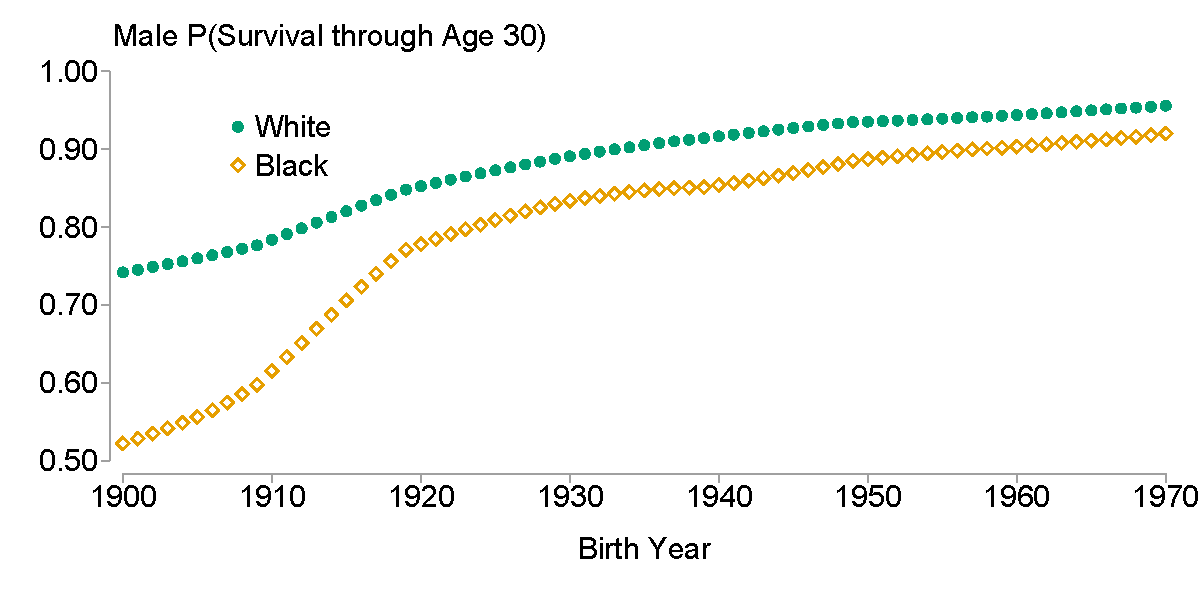
\includegraphics[width=0.8\textwidth]{../analysis/output/figures/figure_1_survivorship_age30_by_race.pdf} 
    \Fnote{
        Probability of survival through age $t$ by race and birth cohort computed from survival probabilities for a hypothetical period life table cohort that experiences the age-specific death rates of the actual population in a given year. 
        See Section~\ref{sec:survivorship} for more details. 
        Source: Period survival probabilities are  taken directly from the CDC data \citepMain{arias_united_2015}. 
    }
\label{fig:p-survival-30-by-race}
\end{figure}

% Figure 2: Infant mortality by race
\begin{figure}[!ht]
    \caption[Infant Mortality By Race and Birth Year]{Infant Mortality By Race and Birth Year}
    \centering
    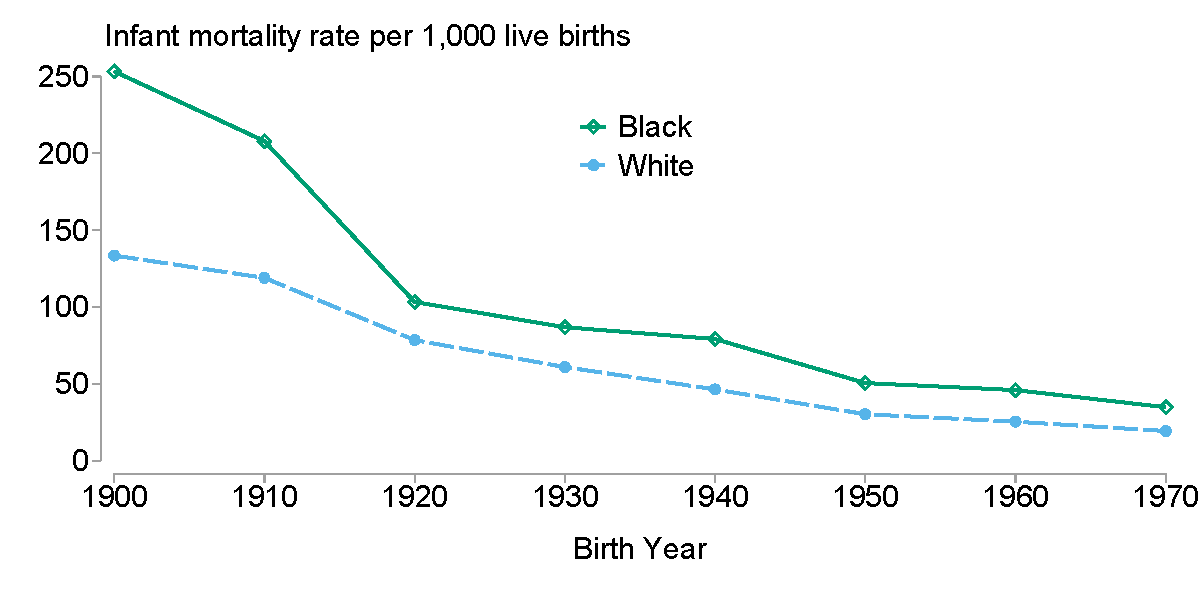
\includegraphics[width=0.8\textwidth]{../analysis/output/figures/figure_2_infant_mortality_by_race.pdf} 
    \Fnote{
        This figure plots Black and white infant mortality rates per 1,000 live births. 
        Birth counts by race are based on published CDC data \citepMain{hamilton_revised_2003}. 
        The number of infant deaths by race are derived from birth counts and the probability of survival from age 0 to 1 taken directly from CDC data \citepMain{arias_united_2015}.
    }
\label{fig:infant-mortality-by-race}
\end{figure}

\restoregeometry

% Figure 3: Life expectancy by race
\begin{figure}[!ht]
    \caption[Male Life Expectancy by Race and Birth Year]{Life Expectancy by Race and Birth Year}
    \centering
    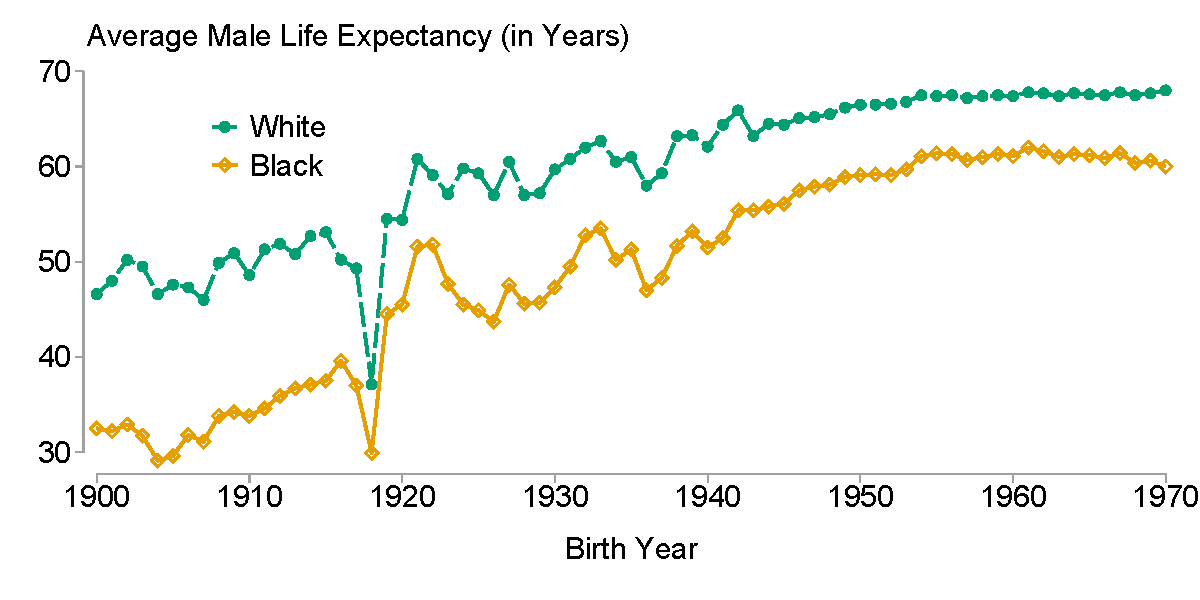
\includegraphics[width=\textwidth]{../analysis/output/figures/figure_3_life_expectancy_by_race.pdf} 
    \Fnote{
        Life expectancy taken directly from CDC data \citepMain{national_center_for_health_statistics_nchs_2015}. 
        The life expectancy measures are calculated using each year's mortality rates for each cohort. 
        See \citeMain{arias_united_2015} for details. 
    }
\label{fig:life-expectancy-by-race}
\end{figure}

% Figure 4: Cross-sectional earnings
\FloatBarrier
\newpage
\newgeometry{top = 0.75in, bottom = 0.75in, right = 0.75in, left = 0.75in, footskip = 0.0in}
\begin{figure}[!ht]
    \caption[White-to-Black Ratio of Average Earnings]{White-to-Black Ratio of Average Earnings}
    \centering
    \begin{subfigure}[b]{0.9\linewidth}
        \centering
        \caption{By Birth Year for 3 Age Groups}
        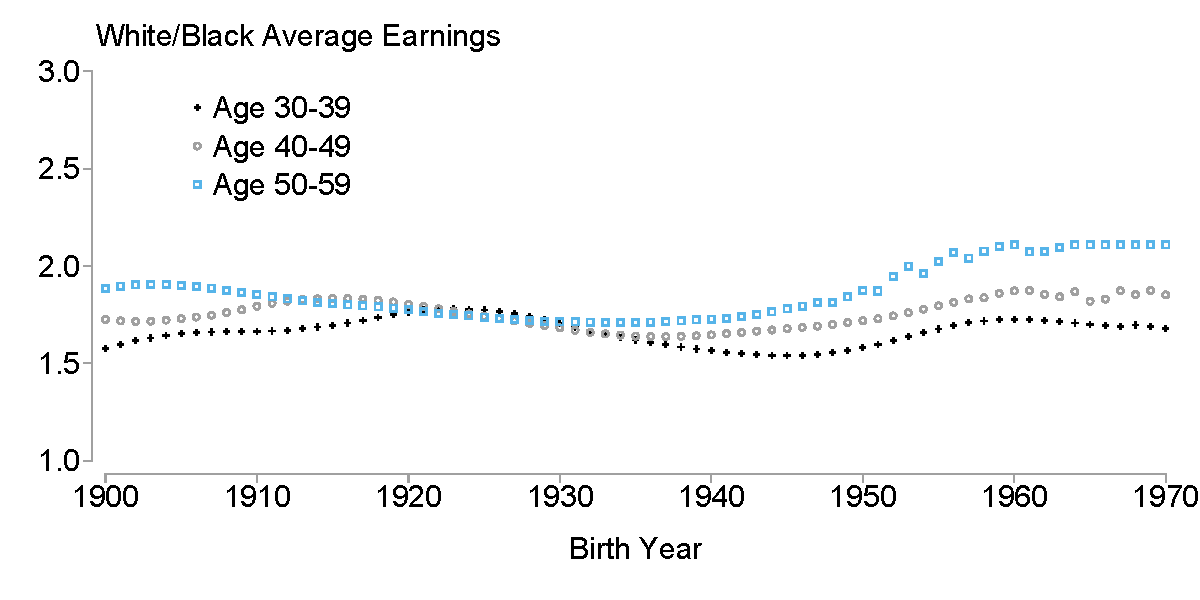
\includegraphics[width=\textwidth]{../analysis/output/figures/figure_4a_bw_ratio_incwage_by_age.pdf} 
    \end{subfigure}
    \begin{subfigure}[b]{0.9\linewidth}
        \centering 
        \caption{By Age for 4 Birth Years}
        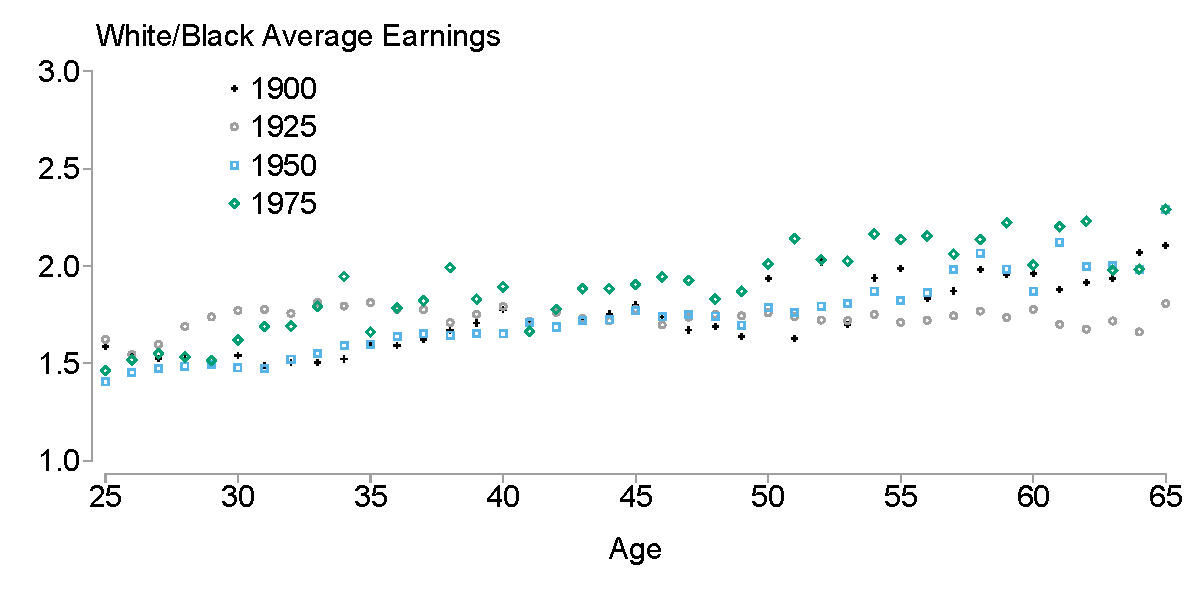
\includegraphics[width=\textwidth]{../analysis/output/figures/figure_4b_bw_ratio_incwage_by_cohort.pdf} 
    \end{subfigure}
    \Fnote{
        See note to Table~\ref{tab:lifetime-earnings-undiscounted}. 
        Earnings are linearly interpolated across race-by-age-by-birth year cells in non-census years and then averaged within 10-year age bins for each birth cohort to produce these scatter plots at an annual level. 
        We assume that earnings after 2014 are equal to earnings in 2014 (within race-by-age cells). 
        This is only relevant for the oldest age group in this figure.
    }
\label{fig:white-black-avg-earnings}
\end{figure}
\restoregeometry


% Figure 5: Lifetime earnings
\FloatBarrier
\newpage
\newgeometry{top = 0.75in, bottom = 0.75in, right = 0.75in, left = 0.75in, footskip = 0.0in}
\begin{figure}[!ht]
    \caption[White-to-Black Ratio of Lifetime Earnings]{White-to-Black Ratio of Lifetime Earnings}
    \centering
    \begin{subfigure}[b]{0.8\linewidth}
        \centering
        \caption{Undiscounted $(\beta=1)$}
        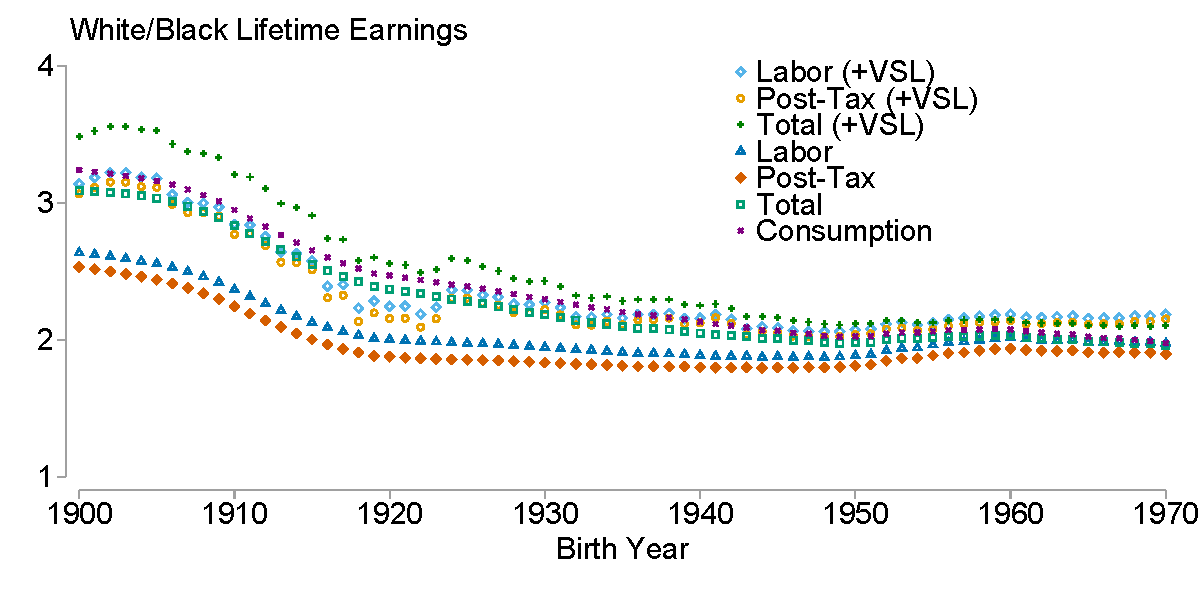
\includegraphics[width=\textwidth]{../analysis/output/figures/figure_5a_wages_lifetime_gaps_discount_100.pdf} 
    \end{subfigure}
    \begin{subfigure}[b]{0.8\linewidth}
        \centering 
        \caption{Discounted $(\beta=0.96)$}
        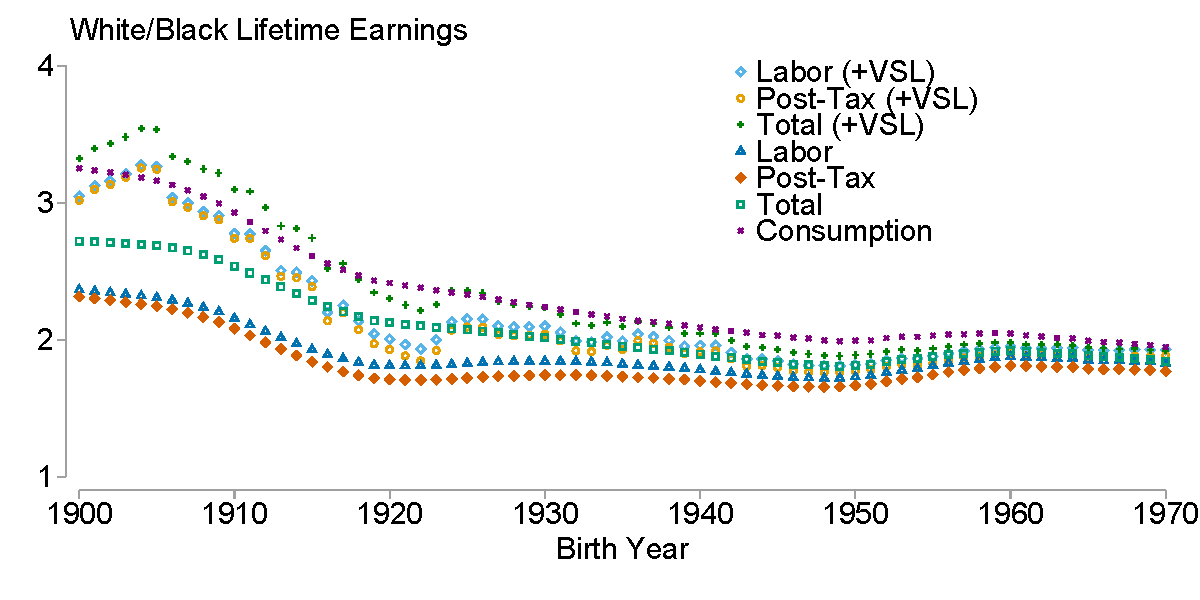
\includegraphics[width=\textwidth]{../analysis/output/figures/figure_5b_wages_lifetime_gaps_discount_096.pdf} 
    \end{subfigure}
    \Fnote{
        See note to Table~\ref{tab:lifetime-earnings-undiscounted}. 
        This figure shows the ratio of white to Black lifetime earnings for each birth cohort. 
        Earnings are undiscounted $(\beta = 1)$ in Panel A and discounted $(\beta = 0.96)$ in Panel B. 
        The +VSL lines correspond to the thought experiment we describe in the text, where we take the ratio of undiscounted white lifetime earnings + the value of the additional life-years each white male can expect to receive to undiscounted Black lifetime earnings. 
        The consumption line corresponds to the lifetime expected consumption of white males divided by the lifetime expected consumption of Black males born in each birth cohort. 
        Here, consumption is calculated assuming $\beta=1$, but this ratio is quite similar when the consumption line is calculated using $\beta=0.96$.
    }
\label{fig:white-black-lifetime-earnings}
\end{figure}
\restoregeometry


% Figure 6: Birth counts
\begin{figure}[!ht]
    \caption[Validation of Survivorship Rates: Raw vs. Implied Birth Counts by Race]{Validation of Survivorship Rates: Raw vs. Implied Birth Counts by Race}
    \centering
    \begin{subfigure}[b]{0.85\linewidth}
        \centering
        \caption{Black males}
        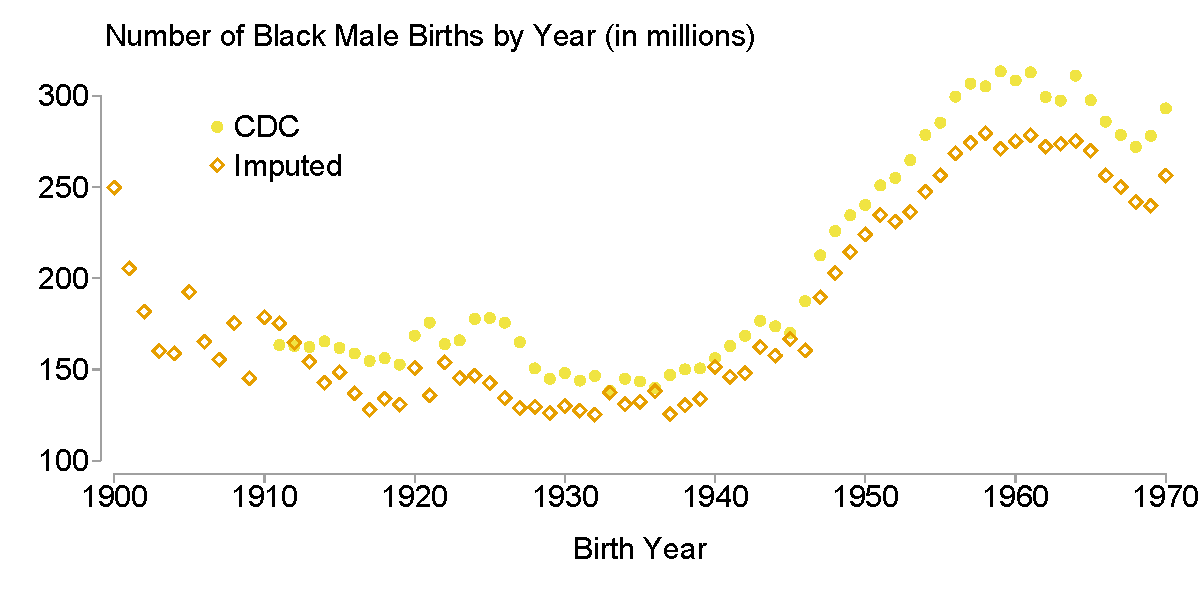
\includegraphics[width=\textwidth]{../analysis/output/figures/figure_6a_birthcounts_blacks.pdf} 
    \end{subfigure}
    \begin{subfigure}[b]{0.85\linewidth}
        \centering 
        \caption{White males}
        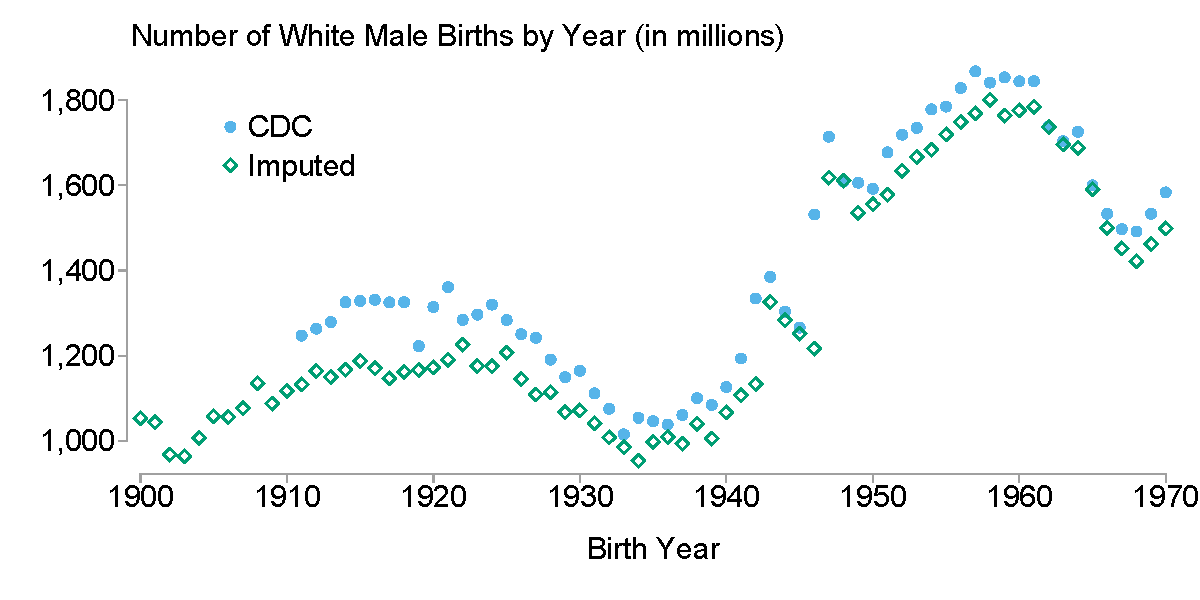
\includegraphics[width=\textwidth]{../analysis/output/figures/figure_6b_birthcounts_whites.pdf} 
    \end{subfigure}
    \Fnote{
        CDC birth counts for Black (panel A) and white (panel B) males based on published CDC data \citepMain{hamilton_revised_2003}. 
        Imputed birth counts apply age-specific mortality rates to birth counts from census microdata \citepMain{IPUMSUSA2023,IPUMSUSA2024}. 
        The imputed data point for each birth year equals the median imputed birth count from age 5-60 census age groups.
    }
\label{fig:birth-counts-by-race}
\end{figure}


% Figure 7: Utility gaps - undiscounted
\FloatBarrier
\newpage
\newgeometry{top = 0.75in, bottom = 0.75in, right = 0.75in, left = 0.75in, footskip = 0.0in}
\begin{figure}[!ht]
    \caption[Undiscounted White and Black Utility by Birth Cohort $(\beta = 1)$]{Undiscounted White and Black Utility by Birth Cohort $(\beta = 1)$}
    \centering
    \begin{subfigure}[b]{0.9\linewidth}
        \centering
        \caption{White and Black Utility in Levels}
        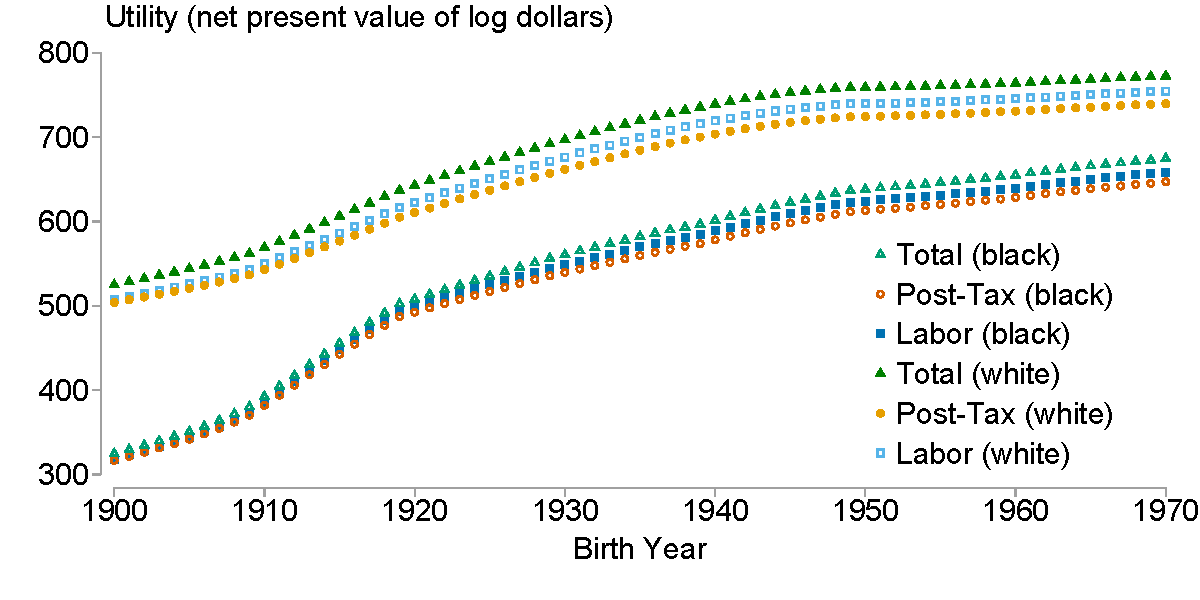
\includegraphics[width=\textwidth]{../analysis/output/figures/figure_7a_utility_by_race_discount_100.pdf} 
    \end{subfigure}
    \begin{subfigure}[b]{0.9\linewidth}
        \centering 
        \caption{White-Black Utility Gap}
        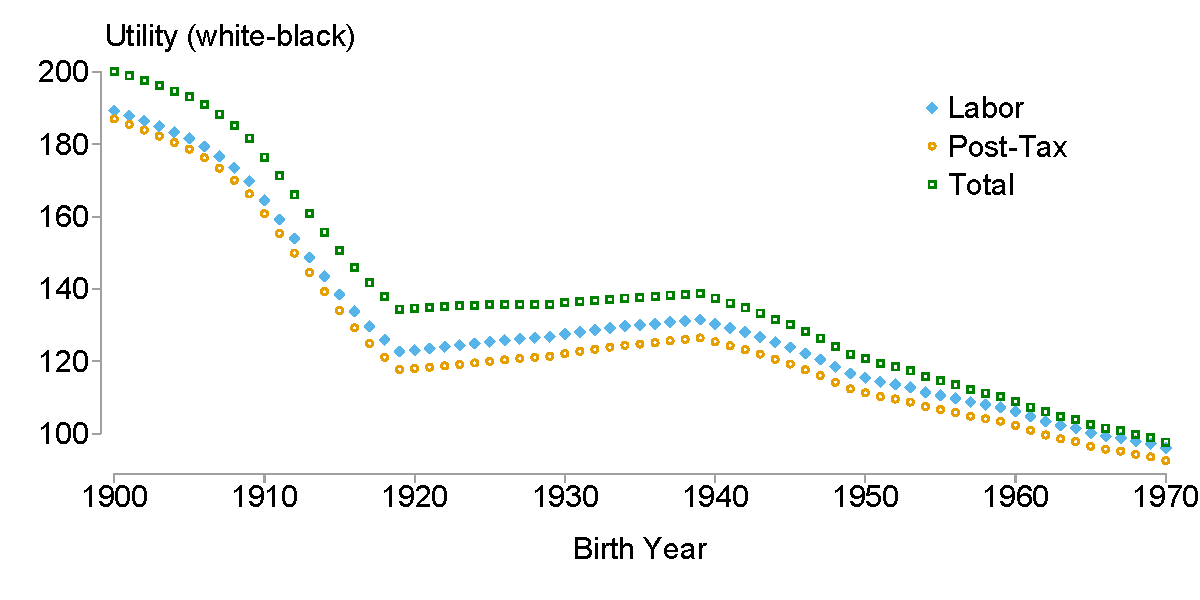
\includegraphics[width=\textwidth]{../analysis/output/figures/figure_7b_utility_gaps_discount_100.pdf} 
    \end{subfigure}
    \Fnote{
        In Panel A, each line is the level of utility for white or Black males, extracted from the structural model we calibrate in the paper. 
        Earnings are not discounted $(\beta = 1)$. 
        Panel B is simply the level difference in white and Black utility from Panel A. 
        We include it to emphasize the large convergence in white and Black utility between the 1900 and 1920 birth cohorts, followed by general stagnation.
    }
\label{fig:white-black-utility-undiscounted}
\end{figure}
\restoregeometry

% Figure 8: Utility gaps - discounted
\FloatBarrier
\newpage
\newgeometry{top = 0.75in, bottom = 0.75in, right = 0.75in, left = 0.75in, footskip = 0.0in}
\begin{figure}[!ht]
    \caption[Discounted White and Black Utility by Birth Cohort $(\beta = 0.96)$]{Discounted White and Black Utility by Birth Cohort $(\beta = 0.96)$}
    \centering
    \begin{subfigure}[b]{0.9\linewidth}
        \centering
        \caption{White and Black Utility in Levels}
        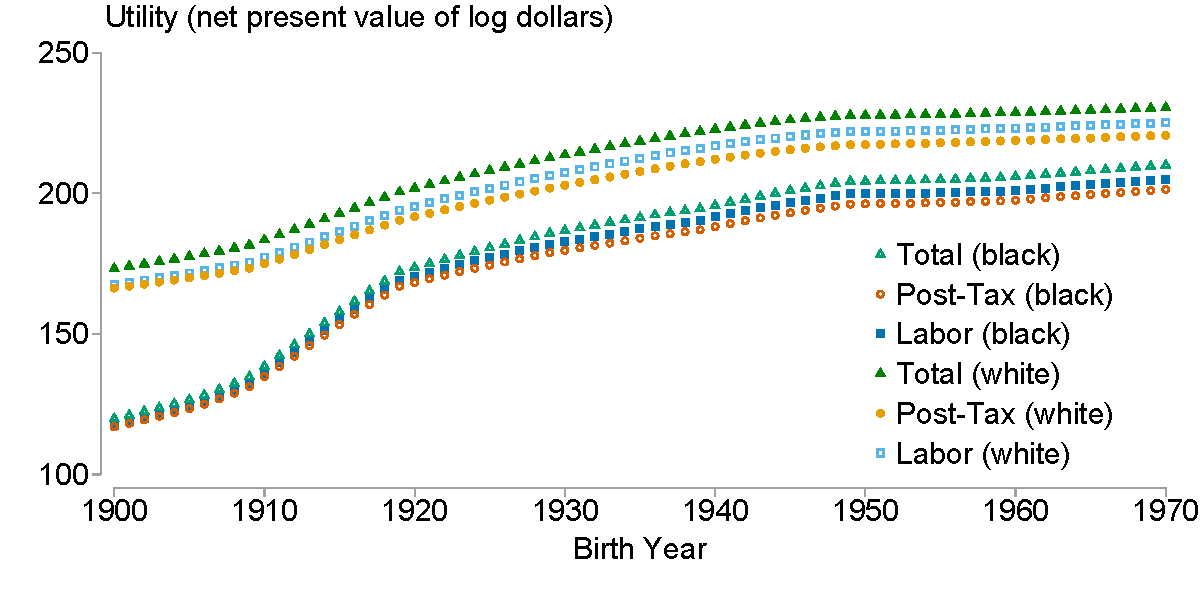
\includegraphics[width=\textwidth]{../analysis/output/figures/figure_8a_utility_by_race_discount_096.pdf} 
    \end{subfigure}
    \begin{subfigure}[b]{0.9\linewidth}
        \centering 
        \caption{White-Black Utility Gap}
        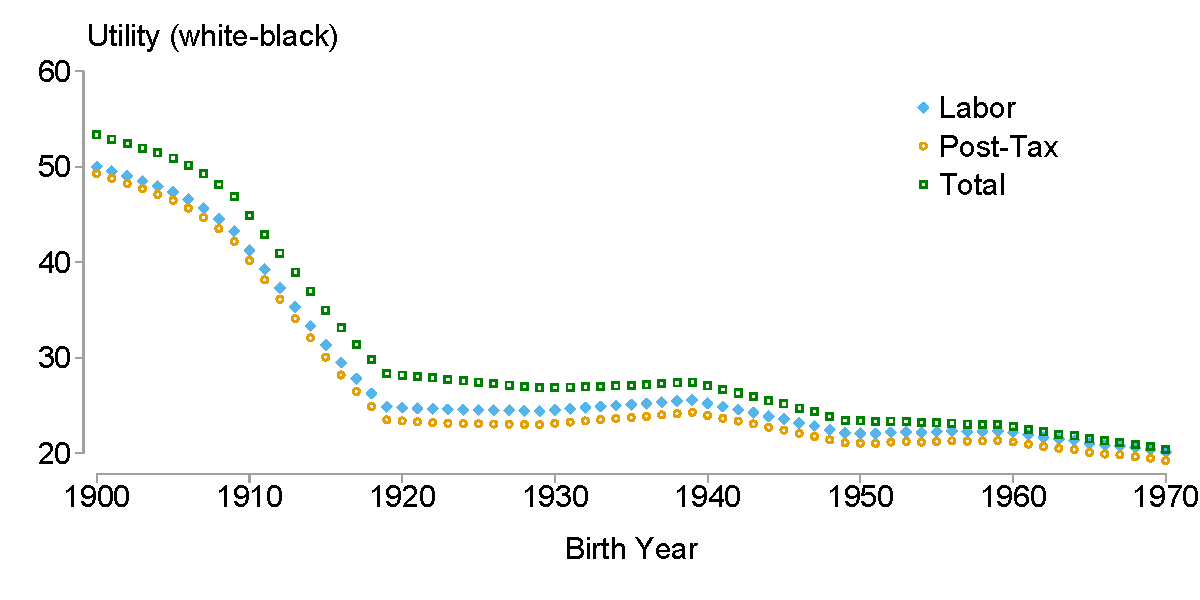
\includegraphics[width=\textwidth]{../analysis/output/figures/figure_8b_utility_gaps_discount_096.pdf} 
    \end{subfigure}
    \Fnote{
        In Panel A, each line is the level of utility for white or Black males, extracted from the structural model we calibrate in the paper. 
        We assume a discount rate of $\beta=0.96$.
        Panel B is simply the level difference in white and Black utility from Panel A. 
        We include it to emphasize the large convergence in white and Black utility between the 1900 and 1920 birth cohorts, followed by general stagnation.
    }
\label{fig:white-black-utility-discounted}
\end{figure}
\restoregeometry

% Figure 9: Robustness
\FloatBarrier
\newpage
\newgeometry{top = 0.75in, bottom = 0.75in, right = 0.75in, left = 0.75in, footskip = 0.0in}
\begin{figure}[!ht]
    \caption[Robustness of White-Black Lifetime Earnings Gap and Utility Gap Estimates]{Robustness of White-Black Lifetime Earnings Gap and Utility Gap Estimates}
    \centering
    \begin{subfigure}[b]{0.9\linewidth}
        \centering
        \caption{White-Black Lifetime Earnings Gap}
        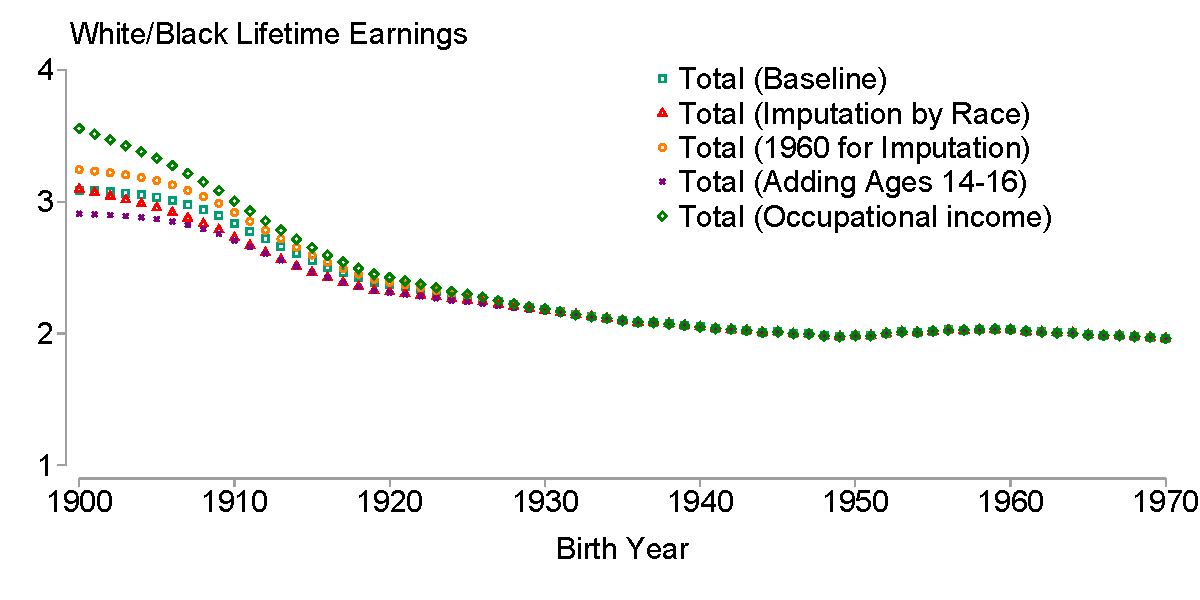
\includegraphics[width=\textwidth]{../analysis/output/figures/figure_9a_wages_lifetime_gaps_robustness_discount_100.pdf} 
    \end{subfigure}
    \begin{subfigure}[b]{0.9\linewidth}
        \centering 
        \caption{White-Black Utility Gap}
        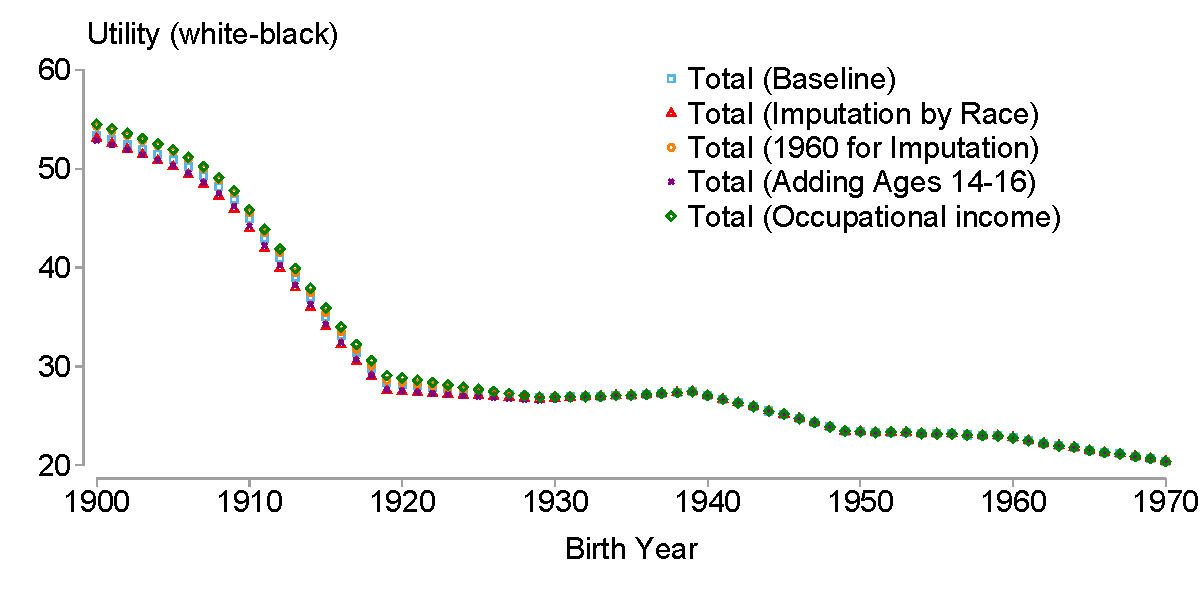
\includegraphics[width=\textwidth]{../analysis/output/figures/figure_9b_utility_gaps_robustness_discount_096.pdf} 
    \end{subfigure}
    \Fnote{
        Panel A shows the White-Black gap in total lifetime income for each birth cohort across various specification choices. 
        The ``Baseline'' specification reproduces the estimates shown in Figure~\ref{fig:white-black-lifetime-earnings}. 
        The ``Imputation by Race'' specification modifies the imputation of non-wage earnings in 1940 and both wage income and non-wage earnings in 1910 to 1930 by interacting all model covariates with an indicator for race. 
        The ``1960 for Imputation'' specification uses the 1960 census to impute non-wage earnings in 1940 rather than the 1950 census. 
        The ``Adding Ages 14-15'' specification includes earnings at ages 14-15 in the lifetime earnings calculation, rather than starting at age 16. 
        The ``Occupational income'' specification uses the average occupational income by race and region in 1960 from \citeMain{collins_african_2022} to impute total income in 1910 to 1940. 
        See Appendix~\ref{sec:app-imputation} for more details on the imputation procedures. 
    }
\label{fig:robust-lifetime-utility}
\end{figure}
\restoregeometry

%------------------------------------------%
%               Appendix
%------------------------------------------%
\FloatBarrier
\appendix
\singlespacing

% Restart page count
\setcounter{page}{1}

\renewcommand*{\thepage}{A\arabic{page}}

\FloatBarrier
\begin{center}
{\Large Appendix: For Online Publication}
 ~\\ ~\\
\noindent{\large \textbf{The Black-White Lifetime Earnings Gap}}
 ~\\ ~\\
\noindent{Ezra Karger and Anthony Wray}
\end{center}

%-------------------------------------------------------------------%
%                Appendix A - Imputation of Earnings
%-------------------------------------------------------------------%

\FloatBarrier
\newpage
\section{Imputation of Earnings \label{sec:app-imputation}}
\setcounter{table}{0}\renewcommand{\thetable}{\ref{sec:app-imputation}\arabic{table}}
\setcounter{figure}{0}\renewcommand{\thefigure}{\ref{sec:app-imputation}\arabic{figure}}
\singlespacing

\paragraph{Pre-processing of data} 
In this appendix section we describe the process used for the imputation of earnings for years where we do not observe earnings data. 
We use the complete-count 1940 US Census and the 5\% sample of the 1950 census from IPUMS, restricting the sample to Black and White males. 
Prior to imputing earnings, we assign zero wage income to all individuals enumerated as prisoners in the 1940 census, to be consistent with other census years. 
We also adjust for inflation by converting nominal earnings to constant 1999 dollars using the IPUMS CPI99 variable (\href{https://usa.ipums.org/usa/cpi99.shtml}{https://usa.ipums.org/usa/cpi99.shtml}). 
We then adjust the base year to 2014 dollars by dividing by a factor of 0.704.

\paragraph{A predictor for negligible non-wage income}
We define non-wage income in 1950 as the difference between total income and wage income. 
We then define \emph{negligible} non-wage income as non-wage income in the range $[-5,5]$ dollars.
Next, we estimate a model for whether an individual has negligible non-wage income in 1950:

\begin{equation}
    \textbf{1}(\text{Negligible Non-Wage Income}_{i} = 1) = \alpha + \gamma_r + \delta_a + \theta_o + \phi_n + \pi_b + \chi_s + \epsilon_i \label{eq:negligible-non-wage-income}
\end{equation}

\noindent where $\gamma_r$ are fixed effects for race, $\delta_a$ are fixed effects for age, $\theta_o$ are fixed effects for occupation (\emph{OCC1950} codes), $\phi_n$ are fixed effects for industry (\emph{IND1950} codes), $\pi_b$ are fixed effects for state of birth, and $\chi_s$ are fixed effects for state of residence. 
We use this model to predict whether an individual has negligible non-wage income in 1940. In combination with the fitted values from this model, we construct a categorical variable for the ventiles of predicted non-wage income across all individuals in the 5\% sample of the 1950 census and the 100\% sample of the 1940 census.
We also construct a categorical variable for the ventiles of wage income across the pooled 1940 and 1950 sample and use these two categorical variables as predictors when imputing 1940 non-wage income.

\paragraph{Imputation of non-wage earnings in 1940} We estimate a model for non-wage earnings in 1950:

\begin{eqnarray}
    \text{Non-Wage Income}_{i}  &=& \alpha + \sum_{p=1}^{20} \beta_p 1(\text{Ventile of predicted non-wage income} = p) \nonumber \\
                                &+& \sum_{q=1}^{20} \eta_q 1(\text{Ventile of wage income} = q) \nonumber  \\
                                &+& \gamma_r + \delta_a + \theta_o + \phi_n + \pi_b + \chi_s + \epsilon_i \label{eq:non-wage-income}
\end{eqnarray}

\noindent where the ventiles of predicted non-wage income, ventiles of wage income and fixed effects are defined above. 
Using this model, we predict non-wage income in 1940 and add to this value the reported wage income in the 1940 census to obtain an estimate of total income in 1940.

\paragraph{Imputation of earnings in 1910 to 1930} Now we impute wage income and total income in the 1910 to 1930 censuses based on the wage income and estimated total income from 1940. 
We modify the model in Equation~\ref{eq:negligible-non-wage-income} to additionally use unemployment status in 1940 as a predictor. 
We proxy for unemployment status in 1940 by using an indicator for \emph{negligible} wage income variable in the 1940 census (i.e. reported wage income in the range $[-5,5]$). 
We use this model to predict whether an individual is unemployment in 1940. In combination with the fitted values from this model, we construct a categorical variable for the ventiles of predicted unemployment status across all individuals in the 5\% sample of the 1950 census and the 100\% sample of the 1940 census. 
We then incorporate the ventiles of predicted unemployment status as a predictor when imputing 1910-1930 wage income in the following equation:

\begin{eqnarray}
    \text{Type of pre-1940 Income}_{i}  &=& \alpha + \sum_{p=1}^{20} \beta_p 1(\text{Ventile of predicted unemployment status} = p) \nonumber \\
                                &+& \gamma_r + \delta_a + \theta_o + \phi_n + \pi_b + \chi_s + \epsilon_i \label{eq:pre-1940-income}
\end{eqnarray}

\noindent where $\text{Type of pre-1940 Income}$ is either wage income or total income. 
Using these models, we predict wage income and total income in 1910, 1920, and 1930. 

\paragraph{Robustness}
In Section~\ref{sec:robustness}, we explore the robustness of our main results to variations on the strategy for the imputation of earnings. 
Here we provide additional details on the adjustments to the imputation procedure. 
In separate specifications, we do the following:
\begin{enumerate}
    \item Modify the prediction models (Equations~\ref{eq:negligible-non-wage-income} to \ref{eq:pre-1940-income}) by incorporating interactions of race with all other fixed effects.  
    \item Use the 5\% sample of the 1960 census rather than the 1\% sample of the 1950 census \citepApp{IPUMSUSA2023} when predicting non-wage income in 1940 due to concerns about small cell sizes in the 1950 census \citepApp{collins_african_2022}. This approach also more closely aligns our income estimates with the occupational earnings score of \citeApp{collins_african_2022} that we implement below. 
    \item Use the 1940 occupational income estimates from \citeApp{collins_african_2022} rather than our imputed earnings for 1910 to 1940. The \citeApp{collins_african_2022} approach imputes 1940 non-wage income using the average non-wage income from the 5\% sample of the 1960 census for each race, region, and occupation cell. We add these estimates to the wage income reported in the 1940 census and apply this measure of total income to all years between 1910 and 1940. In this specification, we do not make any changes to income measures drawn from the 1950 census onward. Our implementation of the \citeApp{collins_african_2022} occupational income score uses the data set provided in the replication package of \citeApp{ward_intergenerational_2023}. See \citeApp{kosack_sueno_2020} and \citeApp{ward_not-so-hot_2020} for more details. 
    \item Include income earned at ages 14 to 15 in our computation of lifetime income. 
\end{enumerate}

%------------------------------------------%
%               Appendix References
%------------------------------------------%
\newpage
\FloatBarrier
%\vspace{1cm}
\setlength{\bibsep}{3pt}

\begin{spacing}{0}
\bibliographystyleApp{references/econ}
{\small\bibliographyApp{references/bw_lifetime_earnings}{}}
\end{spacing}

\end{document}
